% Author	Rajath Shashidhara
% Email		rajath.shashidhara@gmail.com
%
% This work is licensed under the Creative Commons Attribution 4.0 International License. 
% To view a copy of this license, visit http://creativecommons.org/licenses/by/4.0/.

\documentclass[12pt,a4paper,twoside,openany]{report}

\usepackage[width=160mm,top=25mm,bottom=25mm,bindingoffset=6mm,headheight=15pt]{geometry}
\usepackage{cmbright}
% \usepackage[bitstream-charter]{mathdesign}
% \usepackage[urw-garamond]{mathdesign}
% \usepackage{lmodern}
% \usepackage[rm,light]{roboto}
% \usepackage[T1]{fontenc}
% \usepackage{gentium}
% \usepackage[light]{merriweather}

% \usepackage{mathpazo} % math & rm
% \linespread{1.05}        % Palatino needs more leading (space between lines)
% \usepackage[scaled]{helvet} % ss
% \usepackage{courier} % tt
% \normalfont
% \usepackage[T1]{fontenc}

\usepackage{array}
\usepackage{sectsty}
\usepackage{parskip}
\usepackage{fancyhdr}
\usepackage[toc,page]{appendix}

\usepackage{graphicx}
\usepackage{xcolor}
\usepackage{hyperref}
\usepackage[english]{babel}
\usepackage{csquotes}
\usepackage{blindtext}
\usepackage[font={small,it}]{caption}

\usepackage{bigints}
\usepackage{amsmath}
\usepackage{amssymb}
\usepackage{amsthm}
\usepackage{bm}

\usepackage{braket}

\usepackage[backend=biber,style=phys]{biblatex} %AIP style
% \usepackage[backend=biber,style=phys,articletitle=false,biblabel=brackets,chaptertitle=false,pageranges=false]{biblatex}  %APS style
\addbibresource{./bibliography/ref.bib}

%Fix bold fonts in mathmode
%
\DeclareFontFamily{OT1}{cmbr}{\hyphenchar\font45 }
\DeclareFontShape{OT1}{cmbr}{m}{n}{%
  <-9>cmbr8
  <9-10>cmbr9
  <10-17>cmbr10
  <17->cmbr17
}{}
\DeclareFontShape{OT1}{cmbr}{m}{sl}{%
  <-9>cmbrsl8
  <9-10>cmbrsl9
  <10-17>cmbrsl10
  <17->cmbrsl17
}{}
\DeclareFontShape{OT1}{cmbr}{m}{it}{%
  <->ssub*cmbr/m/sl
}{}
\DeclareFontShape{OT1}{cmbr}{b}{n}{%
  <->ssub*cmbr/bx/n
}{}
\DeclareFontShape{OT1}{cmbr}{bx}{n}{%
  <->cmbrbx10
}{}
%


\sectionfont{\fontsize{13}{16}\selectfont}
\subsectionfont{\fontsize{12}{15}\selectfont}

\fancyhead[RE,LO]{\fontsize{6}{9} \selectfont\leftmark}
\fancyhead[RO,LE]{\fontsize{7}{10} \selectfont\rightmark}
\fancyfoot[CO,CE]{\thepage}
\hypersetup{
  colorlinks=true
}

\graphicspath{{./images/},{./figures/}}
\pagestyle{fancy}

\theoremstyle{definition}	\newtheorem{theorem}{Theorem}[section]

\begin{document}
  % Author	Rajath Shashidhara
% Email		rajath.shashidhara@gmail.com
%
% This work is licensed under the Creative Commons Attribution 4.0 International License. 
% To view a copy of this license, visit http://creativecommons.org/licenses/by/4.0/.

\begin{titlepage}
  \begin{center}
    \vspace*{1cm}
    
    \LARGE
    \textbf{Hall conductivity of Aubry-Andr\'e system \\driven by rapidly oscillating magnetic field}
    \vspace{1.5cm}
    \large
    \\ Rajath Shashidhara\\    
    2012B5A7589P\\ \normalsize
    \url{rajath.shashidhara@gmail.com}
    
    \vspace{3.5cm}
    \large
    \textbf{Master Thesis} \\
    \vspace{0.4cm}
    submitted in partial fulillment of the requirements of\\
    BITS F421T Thesis\\
    
    \normalsize
    \vspace{2.5cm}
    Under the supervision of\\
    \vspace{0.2cm}
    \large
    Dr. Tapomoy Guha Sarkar\\
    
    \normalsize
    \vfill
    
\includegraphics[width=0.28\textwidth]{logo.png}
    \vspace{0.5cm}\\
    Department of Physics\\
    Birla Institute of Technology and Science, Pilani\\
    \today
  \end{center}
\end{titlepage}

\normalsize

\newpage
\thispagestyle{empty}

%placeholder text
\begin{abstract}
Study of quantum hall effect in 2D square lattice driven by oscillatory magnetic field perpendicular to the plane.
The time-dependent hamiltonian is solved in fourier space using Brillouin-Wigner perturbation theory, in the high frequency limit.
Investigation of localization/delocalization transitions of time-averaged wavefunctions and calculation of hall conductivity of 
the system using TKNN invariant. Comparison of the results with the effective static hamiltonian picture carried out in the 
previous work.
\end{abstract}

\thispagestyle{empty}

\begin{center}
 \LARGE
 Acknowledgements
\end{center} \normalsize \vspace{2.0cm}
\blindtext
\vfil

\clearpage
\thispagestyle{empty}
\begin{center}
  \LARGE
  Declaration
\end{center} \normalsize \vspace{2.0cm}
I, Rajath Shashidhara, declare that this thesis titled, 
'Hall conductivity of Aubry-Andr\'e system driven by rapidly oscillating magnetic field' and 
the work presented in it is my original work. I affirm that all references are clearly attributed and 
any collaboration with others has been duly acknowledged.
\vspace{5.0cm}\\
\rule[1em]{25em}{0.5pt}\\
(Signature) \vspace{0.5cm}\\
Date: \today \\
\vfil

\clearpage
\thispagestyle{empty}

\begin{center}
  \LARGE
  Certificate
\end{center} \normalsize \vspace{2.0cm}
This is to certify that the thesis titled,  
'Hall conductivity of Aubry-Andr\'e system driven by rapidly oscillating magnetic field' and submitted by
 Rajath Shashidhara 2012B5A7589P in partial fulfillment of the requirements of BITS F421T embodies the work done
 by him under my supervision.\\
\vspace{5.0cm}\\
\rule[1em]{25em}{0.5pt}\\
\large
\emph{Supervisor} \vspace{0.5cm}\\
Dr. Tapomoy Guha Sarkar\\
\normalsize
Department of Physics\\
Birla Institute of Technology and Science, Pilani \vspace{0.5cm}\\
Date: \today \\
\vfil
\tableofcontents
  % Author	Rajath Shashidhara
% Email		rajath.shashidhara@gmail.com
%
% This work is licensed under the Creative Commons Attribution 4.0 International License. 
% To view a copy of this license, visit http://creativecommons.org/licenses/by/4.0/.

\chapter{Introduction}
% \section{section}
% \subsection{subsection}

  \part{Background}
  % Author	Rajath Shashidhara
% Email		rajath.shashidhara@gmail.com
%
% This work is licensed under the Creative Commons Attribution 4.0 International License. 
% To view a copy of this license, visit http://creativecommons.org/licenses/by/4.0/.

\chapter{Geometric Phase}
Physical measurements or observations are extracted from quantum mechanical systems in the form of expectation values of hermitian operators $\braket{\psi|\hat{A}|\psi}$.
Eigenvectors of the hamiltonian are only specified up to a phase factor. Expectation values and thereby, the physical observations are unaltered by a transformation of the form 
$\psi \rightarrow e^{i \phi} \psi$. Gauge-dependent quantities are considered unphysical and the phase of the eigenvectors is usually thrown away from analysis. Berry
demonstrated the existence of a gauge-invariant phase called the geometric phase - a physically observable quantity.
% This guage choice can be eliminated by formulating quantum mechanics in terms of guage invariant representations such as density 
% matrices $\psi\psi^{\dagger}$. Expectation value of an operator $\hat{A}$ is recast as $\braket{\hat{A}} = tr(\psi\psi^{\dagger}\hat{A})$.

\section{Definition}
Prof. M V Berry studied the adiabatic evolution of a quantum system described by the hamiltonian $\hat{H}(\mathbf{R})$, parameterized by external factors $\mathbf{R}$ -- such as
magnetic field, electric field, etc \cite{berry1984quantal}. The hamiltonian is varied by slowly changing $\mathbf{R}$ from time $t=0$ to $t=T$ such that $\mathbf{R}(0)=\mathbf{R}(T)$. This evolution is
a closed loop in the parameter space. Apart from the adiabatic assumption, we also assume that the energy spectrum is discrete and there are no level crossings or degeneracies in the 
energy spectrum. Using the guage freedom, we enforce single-valuedness on the eigenvectors of the hamiltonian in the parameter space. 
Under the assumptions stated above, eigenvectors of the hamiltonian can be uniquely identified as $\ket{n(\mathbf{R})}$ at each point in parameter space without any ambiguity.
The schrodinger equation is stated in this notation as 
\begin{gather}
 \hat{H}(\mathbf{R}(t))\ket{n(\mathbf{R}(t))} = E(\mathbf{R}(t))\ket{n(\mathbf{R}(t))} \\
 \label{chap_2:timedepschroeq} i\hbar\frac{\partial}{\partial t}\ket{\psi(t)} = \hat{H}(t)\ket{\psi(t)}
\end{gather} In the case of static time-independent hamiltonian, any state expanded as a linear combination of stationary states is written as
$\ket{\psi(t)} = \sum{c_n e^{-\frac{i E_{n}(t)}{\hbar}} \ket{n}}$. Taking cue from this, the expansion ansatz
\begin{equation}
\ket{\psi(t)} = \sum{c_{n}(t) e^{-\frac{i}{\hbar}\int_{0}^{t}{E_{n}(t) dt}} \ket{n(t)}}
\end{equation} is a valid generalization for a system with a time-dependent hamiltonian. When the ansatz is substituted into Eq. \eqref{chap_2:timedepschroeq}, we obtain
\begin{equation}
  \label{chap_2:coeffslinercomb}\dot{c}_{m}(t) = -c_{m}(t) \Braket{m(t) | \frac{\partial}{\partial t} m(t)} - \sum_{n}{c_{n}(t) e^{i (\theta_n - \theta_m)} \frac{\braket{m(t)|\widehat{\dot{H}}|n(t)}}{E_n - E_m}}
\end{equation} where $\theta_n = \frac{-1}{\hbar}\int_{0}^{t}{E_n(t')\,dt'}$. In the adiabatic limit, the transition probability between states tends to zero.
We ignore the second term in the general solution above to obtain the result
\begin{equation}
 c_{n}(t) = e^{i \gamma_{n}(t)}\,c_{n}(0)
\end{equation} If we started in an eigenstate of the hamiltonian $\ket{\psi(0)} = \ket{n(\mathbf{R}(0)}$, then the state evolves as
\begin{equation}
 \ket{\psi(t)} = e^{i \gamma_{n}(t)} e^{i \theta_{n}(\mathbf{R}(t))} \ket{n(\mathbf{R}(t))}
\end{equation} remaining in the $n$th eigenstate all along, only picking up phase factors. In the case of cyclic evolution, we write
\begin{equation}
 \ket{\psi(T)} = e^{i \gamma_{n}(C)} e^{i \theta_{n}(T)} \ket{\psi(0)}
\end{equation}
From Eq. \eqref{chap_2:coeffslinercomb}, we note that
\begin{equation}
  \gamma_{n}(C) = i\,\int_{0}^{T}{\braket{n(t) | \frac{\partial}{\partial t} n(t)}\, dt} = i\, \oint_{c}{\braket{n(\mathbf{R})| \bm{\nabla_{R}} | n(\mathbf{R})} \cdot \, d\mathbf{R}}
\end{equation} $\gamma_{n}(C)$ is a real number and therefore $e^{i \gamma_{n}(C)}$ is a pure phase term. This simple fact can be demonstrated by taking the time-derivative 
of $\braket{n(t)|n(t)} = 1$.
\begin{gather*}
 \braket{n(t)|n(t)} = 1 \\
 \left[\frac{\partial}{\partial t}\bra{n(t)}\right]\ket{n(t)} + \bra{n(t)}\left[ \frac{\partial}{\partial t}\ket{n(t)}\right] = 0 \\
 \bra{n(t)}\left[\frac{\partial}{\partial t}\ket{n(t)}\right] = -\left(\bra{n(t)}\left[\frac{\partial}{\partial t}\ket{n(t)}\right]\right)^{*}
\end{gather*}
$\theta_{n}(T)$ is the familiar dynamical phase and $\gamma_{n}(C)$ is known as geometric phase or simply berry phase. While the dynamical phase is a time-dependent quantity,
the geometric phase is a line integral, that only depends on path traversed in the parameter space. Another important observation is the fact that $\gamma_{n}$ is a 
non-integrable quantity as it is not single valued - $\gamma_{n}(0) \neq \gamma_{n}(T)$ in the parameter space. Therefore, the geometric phase cannot be expressed as a field over
the parameter space. By application of stokes theorem, the line integral can be convereted into a surface integral as shown below
\begin{align}
 \gamma_{n}(C) &= i \oint_{C}{\braket{n(\mathbf{R})| \bm{\nabla_{R}} | n(\mathbf{R})} \cdot \, d\mathbf{R}} \nonumber \\
 &= i \int_{S}{\bm{\nabla_{R}} \wedge \braket{n(\mathbf{R})| \bm{\nabla_{R}} | n(\mathbf{R})} \cdot \, d\mathbf{S}} \\
 &= i \int_{S}{(\bm{\nabla_{R}}\bra{n(\mathbf{R})}) \wedge \bm{\nabla_{R}}\ket{n(\mathbf{R})} \cdot \, d\mathbf{S}} \nonumber \\
 \label{chap_2:gaugeindep} &= i \bigintsss_{S}{\,\sum_{m \neq n}{\frac{\braket{n(\mathbf{R})|\bm{\nabla_{R}}\hat{H}(\mathbf{R})|m(\mathbf{R})} \wedge \braket{m(\mathbf{R})|\bm{\nabla_{R}}\hat{H}(\mathbf{R})|n(\mathbf{R})}}{(E_{n}(\mathbf{R})- E_{m}(\mathbf{R}))^2}} \cdot \, d\mathbf{S}}
\end{align}
Eq. \eqref{chap_2:gaugeindep} has a remarkable property of being gauge independent. Any transformation of the form 
$\ket{n(\mathbf{R})} \rightarrow e^{i\delta(\mathbf{R})} \ket{n(\mathbf{R})}$, leaves Eq. \eqref{chap_2:gaugeindep} unchanged. 

% \subsection{Anology to electromagnetism}
Before we proceed, it is useful to define two important quantities called the berry connection and the berry curvature. \emph{Berry connection} is defined as
\begin{equation}
 \mathbf{A}_{n}(\mathbf{R}) = i\braket{n(\mathbf{R})| \bm{\nabla_{R}} | n(\mathbf{R})}
\end{equation}
and the \emph{Berry curvature} is given by
\begin{equation}
 \mathbf{B}_{n}(\mathbf{R}) = i \;\bm{\nabla_{R}} \wedge \braket{n(\mathbf{R})| \bm{\nabla_{R}} | n(\mathbf{R})} = \bm{\nabla_{R}} \wedge \mathbf{A}_{n}(\mathbf{R})
\end{equation} Berry phase is conveniently expressed in terms of these quantities as
\begin{equation}
 \gamma_{n}(C)= \oint_{C}{\mathbf{A}_{n}(\mathbf{R})\cdot \, d\mathbf{R}} = \int_{S}{\mathbf{B}_{n}(\mathbf{R})\cdot \, d\mathbf{S}}
\end{equation}
If we transform the states as $\ket{n(\mathbf{R})} \rightarrow e^{i\delta(\mathbf{R})} \ket{n(\mathbf{R})}$, then the berry connection transforms as
$\mathbf{A}_{n}(\mathbf{R}) \rightarrow \mathbf{A}_{n}(\mathbf{R}) - \bm{\nabla_{R}} \delta(\mathbf{R})$, but the berry curvature remains unchanged. This shows an uncanny
resemblance between magnetic vector potential and the berry connection and consequently the magnetic field strength and the berry curvature. However, it must be kept in mind that
the berry connection and the berry curvature are defined over the parameter space (could be more than 4-dimensional) and not the real space.

Geometric phase was overlooked as physically irrelevant as the expectation values are independent of the phase of eigenfunctions. 
As opposed to the then prevalent notion, Prof. Berry, in his seminal paper, demonstrated that the geometric phase is in fact, physically observable \cite{berry1984quantal,wilczek1989geometric}.
Several assumptions imposed by Prof. Berry in defining the geometric phase can be relaxed and definition of geometric phase has been generalized to nonadiabatic, noncyclic, 
nonunitary and nonabelian situations \cite{aharonov1987phase, samuel1988general, wilczek1984appearance, mukunda1993quantum}.

\section{Bargmann invariants}
A remarkable feature of the berry phase is that it is a geometric quantity, i.e., it is a property arising by virtue of the geometry of the 
underlying hilbert space. In \parencite{mukunda1993quantum}, it is demonstrated that the berry phase is both gauge and reparameterization 
invariant (thereby a geometric property) using purely kinematic arguments. Geometric phase is akin to parallel transport of vectors on a 
non-trivial manifold. Just as the co-variant derivative of a vector on a manifold has contributions purely arising from the underlying 
geometry, the geometric phase is acquired by a state evolving in the hilbert space by virtue of its geometry \cite{simon1983holonomy}. 
Precisely, berry phase is the holonomy in a hermitian line bundle in the language of differential geometry.

In this section, our intention is to express the berry phase in terms of gauge invariant quantities called Bargmann invariants. 
Bargmann invariant of order $j$ of a series of $j$ normalized states $\ket{\psi_j}$ such that $\braket{\psi_j|\psi_{j+1}} \neq 0$ is defined as 
\begin{equation}
 \Delta^{(j)}(\psi_1, \dots, \psi_j) = \braket{\psi_1 | \psi_2}\braket{\psi_2|\psi_3}\dots\braket{\psi_{j-1}|\psi_j}\braket{\psi_j|\psi_1}
\end{equation} It is apparent from the definition that $\Delta^{(j)}$ is invariant under a $U(1) \times U(1) \dots j\;times$ transformation.
Consider the space of eigenfunctions parameterized (under the assumptions as 
described in the previous section) by $\mathbf{R}$, the inner product 
\begin{align}
e^{i\Delta\gamma} &= \frac{\braket{n(\mathbf{R})|n(\mathbf{R} +\delta\mathbf{R})}}{|\braket{n(\mathbf{R})|n(\mathbf{R} +\delta\mathbf{R})}|} \\
 		  &\approx \frac{\bra{n(\mathbf{R})}\;\lbrack \ket{n(\mathbf{R})} + \bm{\nabla_R}\ket{n(\mathbf{R})}\cdot \delta\mathbf{R}\, + \dots \rbrack}{|\braket{n(\mathbf{R})|n(\mathbf{R} +\delta\mathbf{R})}|} \nonumber \\
1 + i\Delta\gamma + \dots &\approx \frac{1 + \braket{n(\mathbf{R})|\bm{\nabla_R}|n(\mathbf{R})}\cdot \delta\mathbf{R} + \dots}{|\braket{n(\mathbf{R})|n(\mathbf{R} +\delta\mathbf{R})}|} \nonumber \\
\Delta\gamma	   &\approx  -i\braket{n(\mathbf{R})|\bm{\nabla_R}|n(\mathbf{R})}\cdot \delta\mathbf{R}
\end{align}
We have established that 
\begin{equation*}
 \arg(\braket{n(\mathbf{R})|n(\mathbf{R} +\delta\mathbf{R})}) \approx -\mathbf{A}_{n}(\mathbf{R}) \cdot \delta\mathbf{R}
\end{equation*} which means that
\begin{multline}
 \label{chap_2:geombargmanninv}\gamma(C) = \oint_{C}{\mathbf{A}_{n}(\mathbf{R}) \cdot \delta\mathbf{R}}  = -\oint_{C}{\arg(\braket{n(\mathbf{R})|n(\mathbf{R} +\delta\mathbf{R})})} \\ = -\lim_{N\rightarrow\infty} \arg(\prod_{j=0}^{N-1}{\braket{n(\mathbf{R}(t + j\Delta t))|n(\mathbf{R}(t + (j+1)\Delta t))}})
\end{multline} where $\Delta t = \frac{T}{N} \ni \mathbf{R}(0)=\mathbf{R}(T)$.
Immediately we recognize that the RHS of Eq. \eqref{chap_2:geombargmanninv} is the argument of Bargmann invariant of states lying on the path $C$.

The Berry curvature surface integral can also be expressed in terms of the Bargmann invariant. We derive the relationship below for a 2-dimensional parameter space
labeled by $\bm{\lambda} = (\lambda_x, \lambda_y)$. This result can be easily generalized to arbitrary dimensions. Consider an infinitesimal square $Q$ in the parameter space 
consisting of points $(\lambda_x, \lambda_y), (\lambda_x + \delta\lambda_x, \lambda_y), (\lambda_x + \delta\lambda_x, \lambda_y + \delta\lambda_y), (\lambda_x, \lambda_y+\delta\lambda_y)$
in anti-clockwise order. The integral of berry connection around this closed loop is
\begin{multline*}
  \oint_{Q}{\mathbf{A}_{n}(\bm{\lambda})\cdot \delta\bm{\lambda}} = \\
  -\arg(\braket{n(\bm{\lambda})|n(\bm{\lambda} + \delta\lambda_x \hat{\mathbf{x}})}\braket{n(\bm{\lambda} + \delta\lambda_x \hat{\mathbf{x}})|n(\bm{\lambda} + \delta\lambda_x \hat{\mathbf{x}} + \delta\lambda_y \hat{\mathbf{y}})}\\ \braket{n(\bm{\lambda} + \delta\lambda_x \hat{\mathbf{x}} + \delta\lambda_y \hat{\mathbf{y}})|n(\bm{\lambda} + \delta\lambda_y \hat{\mathbf{y}})}\braket{n(\bm{\lambda} + \delta\lambda_y \hat{\mathbf{y}})|n(\bm{\lambda})})
\end{multline*}
Using stokes theorem
\begin{align*}
  \oint_{Q}{\mathbf{A}_{n}(\bm{\lambda})\cdot \delta\bm{\lambda}} &= \int_{Q}{\mathbf{B}_{n}(\bm{\lambda})\cdot d\mathbf{S}_{\bm{\lambda}}}\\
  &= \mathbf{B}_{n}(\bm{\lambda}) \delta\lambda_x\delta\lambda_y
\end{align*}
Combining these two results, we infer that
\begin{multline}
 \mathbf{B}_{n}(\bm{\lambda}) \delta\lambda_x\delta\lambda_y = \\
 -\arg(\braket{n(\bm{\lambda})|n(\bm{\lambda} + \delta\lambda_x \hat{\mathbf{x}})}\braket{n(\bm{\lambda} + \delta\lambda_x \hat{\mathbf{x}})|n(\bm{\lambda} + \delta\lambda_x \hat{\mathbf{x}} + \delta\lambda_y \hat{\mathbf{y}})}\\ \braket{n(\bm{\lambda} + \delta\lambda_x \hat{\mathbf{x}} + \delta\lambda_y \hat{\mathbf{y}})|n(\bm{\lambda} + \delta\lambda_y \hat{\mathbf{y}})}\braket{n(\bm{\lambda} + \delta\lambda_y \hat{\mathbf{y}})|n(\bm{\lambda})})
\end{multline}
This result is particularly useful when numerically evaluating the surface integral of a berry phase in discretized parameter space.

% The argument of the four-point Bargmann invariant is
% \begin{multline}
% \arg(\braket{n(\bm{\lambda})|n(\bm{\lambda} + \delta\lambda_x \hat{\mathbf{x}})}\braket{n(\bm{\lambda} + \delta\lambda_x \hat{\mathbf{x}})|n(\bm{\lambda} + \delta\lambda_x \hat{\mathbf{x}} + \delta\lambda_y \hat{\mathbf{y}})}\\ \braket{n(\bm{\lambda} + \delta\lambda_x \hat{\mathbf{x}} + \delta\lambda_y \hat{\mathbf{y}})|n(\bm{\lambda} + \delta\lambda_y \hat{\mathbf{y}})}\braket{n(\bm{\lambda} + \delta\lambda_y \hat{\mathbf{y}})|n(\bm{\lambda})}) \\
% = \arg(\braket{n(\bm{\lambda})|n(\bm{\lambda} + \delta\lambda_x \hat{\mathbf{x}})}) + \arg(\braket{n(\bm{\lambda} + \delta\lambda_x \hat{\mathbf{x}})|n(\bm{\lambda} + \delta\lambda_x \hat{\mathbf{x}} + \delta\lambda_y \hat{\mathbf{y}})}) \\ + \arg(\braket{n(\bm{\lambda} + \delta\lambda_x \hat{\mathbf{x}} + \delta\lambda_y \hat{\mathbf{y}})|n(\bm{\lambda} + \delta\lambda_y \hat{\mathbf{y}})}) + \arg(\braket{n(\bm{\lambda} + \delta\lambda_y \hat{\mathbf{y}})|n(\bm{\lambda})}) 
% \end{multline}
% \begin{align}
%  &= -A^{n}_{x}(\bm{\lambda})\delta\lambda_x - A^{n}_{y}(\bm{\lambda} + \delta\lambda_x \hat{\mathbf{x}})\delta\lambda_y + A^{n}_{x}(\bm{\lambda}+ \delta\lambda_x \hat{\mathbf{x}}+ \delta\lambda_y \hat{\mathbf{y}})\delta\lambda_x + A^{n}_{y}(\bm{\lambda} + \delta\lambda_y \hat{\mathbf{y}})\delta\lambda_y \nonumber \\
%  &\text{Using taylor expansion upto $1$ st order,} \nonumber \\
%  &\approx -A^{n}_{x}(\bm{\lambda})\delta\lambda_x - A^{n}_{y}(\bm{\lambda})\delta\lambda_y - \partial_{x}A^{n}_{y}(\bm{\lambda})\delta\lambda_x\delta\lambda_y +A^{n}_{x}(\bm{\lambda})\delta\lambda_x + \partial_{x}A^{n}_{x}(\bm{\lambda})\delta\lambda_x\delta\lambda_x + \partial_{y}A^{n}_{x}(\bm{\lambda})\delta\lambda_x\delta\lambda_y\nonumber \\
%  &+ A^{n}_{y}(\bm{\lambda})\delta\lambda_y + \partial_{y}A^{n}_{y}(\bm{\lambda})\delta\lambda_y\delta\lambda_y \nonumber \\
%  &= - \partial_{x}A^{n}_{y}(\bm{\lambda})\delta\lambda_x\delta\lambda_y - \partial_{x}A^{n}_{x}(\bm{\lambda})\delta\lambda_x\delta\lambda_x + \partial_{y}A^{n}_{x}(\bm{\lambda})\delta\lambda_x\delta\lambda_y+ \partial_{y}A^{n}_{y}(\bm{\lambda})\delta\lambda_y\delta\lambda_y \nonumber \\ 
%  \label{chap_2:bargberry} &= - \partial_{x}A^{n}_{y}(\bm{\lambda})\delta\lambda_x\delta\lambda_y + \partial_{y}A^{n}_{x}(\bm{\lambda})\delta\lambda_x\delta\lambda_y \\
%  &= - \mathbf{B}_{n}(\bm{\lambda}) \cdot d\mathbf{S}_{\bm{\lambda}}
% \end{align}
% We have ignored $\partial_{x}A^{n}_{x}(\bm{\lambda})\delta\lambda_x\delta\lambda_x$ and $\partial_{y}A^{n}_{y}(\bm{\lambda})\delta\lambda_y\delta\lambda_y$ in Eq. \eqref{chap_2:bargberry},
% because they are purely imaginary and the higher order contributions from the taylor series expansion will cancel them. This is guaranteed, because we have already proven
% that the berry connection is a real number. Below is a proof of $\partial_{x}A^{n}_{x}(\bm{\lambda})\delta\lambda_x\delta\lambda_x$ is imaginary

\section{Non-abelian Berry connection}	
  % Author	Rajath Shashidhara
% Email		rajath.shashidhara@gmail.com
%
% This work is licensed under the Creative Commons Attribution 4.0 International License. 
% To view a copy of this license, visit http://creativecommons.org/licenses/by/4.0/.

\chapter{Quantum Hall Effect}\label{ch:qhe}
It was observed in two-dimensional materials placed in strong magnetic fields, the Hall conductivity is quantized\footnote{Knowledge of Classical Hall effect is assumed in this discussion.
\parencite{kitel1971introduction,tong2016lectures,jain2007composite} contain excellent review of the subject} \cite{klitzing1980new, prange1990quantum, jain2007composite}. The striking feature is that the quantization is robust to disorder and independent of
material or its geometry. Classical conduction theories such as the Drude's model failed to explain this strange phenomenon. 

Eventually, the Landau problem that describes the cyclotron motion of electrons restricted to 2-dimensional plane in the presence of magnetic field was connected with the Quantum Hall effect. 
The energy levels in the Landau problem are quantized, called the Landau levels, each level is degenerate by roughly the magnitude of magnetic flux (magnetic field times the area) passing 
through the sample. The quantization of Hall conductance was linked to the filling fraction of the Landau levels. Although this was successful in explaining the magnitude of Hall
conductance, it failed to explain the robustness of the phenomenon. The idea of edge states and the role of disorder was incorporated into heuristic explanations to explain the plateaus of Hall conductance, based on localization
of states in the presence of disorder. However, if only a fraction of all states are localized, and only the localized states contribute to conduction, the value of Hall conduction as explained
by the filling fraction of Landau levels assuming each state contributed equally to conduction, is in direct contradiction to the idea of localized states. This puzzle was finally cracked by 
Laughlin using the idea of gauge invariance of electromagnetism and the concept of spectral flow \cite{laughlin1981quantized, prange1981quantized, halperin1982quantized, jain2007composite, tong2016lectures}.

The breakthrough result was established by Thouless et al., as they demonstrated that Hall conductivity is indeed a topological invariant which is an integral quantity\footnote{This work was awarded the Nobel prize in 2016 - incidentally the period during which this document was compiled} \cite{thouless1982quantized,kohmoto1985topological,simon1983holonomy}. The topology of the hilbert space parameterized by 
the crystal momentum of the lattice, manifests as the Hall conductance of the material. This explanation supplanted all the previous theories, unveiled the deeper topological links to conduction
and launched a whole branch of physics called topological insulators. We sHall study techniques in this thesis to calculate the topological invariant and identify topological phase transitions
in quantum systems.

\section{Brillouin zone as the parameter space}
Consider a particle moving on a rectangular lattice. By application of bloch theorem, the wavefunction can be factorized as
\begin{equation*}
 \ket{\psi_{\mathbf{k}}(\mathbf{x})} = e^{i\mathbf{x}\cdot\mathbf{x}}\ket{u_{\mathbf{k}}(\mathbf{x})}
\end{equation*} such that $\ket{u_{\mathbf{k}}(\mathbf{x})} = \ket{u_{\mathbf{k}}(\mathbf{x}+\mathbf{R})}$ where $\mathbf{R}$ is a lattice translation vector.
The crystal momentum $\mathbf{k}$ is bounded in the first Brillouin zone\footnote{In the presence of magnetic field, we shall use the magnetic Brillouin zone. See Chapter \ref{ch:aah}.}
\begin{equation*}
 \frac{-\pi}{a} < k_{x} \leq \frac{\pi}{a} \text{ and } \frac{-\pi}{b} < k_{y} \leq \frac{\pi}{b}
\end{equation*} The Hamiltonian $\hat{H}(\mathbf{k})$ is also parametrized by the crystal momentum. The Brillouin zone is a torus $\mathbf{T}^2$ and by changing the parameters
$k_{x}$ and $k_{y}$, we can apply the idea of Berry described in the previous chapter.

\section{Kubo formula for conductivity}
We shall use the Brillouin zone as the arena and calculate the transverse electrical conductivity on a 2D rectangular lattice. Bands are labelled by $\alpha$ and the crystal momentum by $\mathbf{k}$.
The linear response of current in the transverse direction to the applied electric field was derived by Kubo \cite{kubo1956general,kubo1957statistical,tong2016lectures,kohmoto1985topological,thouless1982quantized}.
Kubo's result is a relationship like Ohm's law, the electric field (stimulus) and the current density (response) are correlated linearly as\footnote{At absolute zero $T=0$.}
\begin{gather}
 J_{x} = \sigma_{xy} E_{y} \\
 \sigma_{xy} = i\hbar \sum_{\alpha,\beta | E_{\alpha}<E_{F}<E_{\beta}}\int_{\mathbf{T}^2}\frac{d^2 k}{(2\pi)^2} \frac{\braket{u_k^\alpha |J_{y}|u_k^\beta}\braket{u_k^\beta |J_{x}|u_k^\alpha} - \braket{u_k^\alpha |J_{x}|u_k^\beta}\braket{u_k^\beta |J_{y}|u_k^\alpha}}{(E_{\beta}(\mathbf{k})-E_{\alpha}(\mathbf{k}))^2}
\end{gather}
$E_{F}$ is the Fermi energy.

\section{TKNN Invariant}
Thouless et al. in their seminal paper, using the Kubo formula for electric conductivity, showed that the Hall conductivity of Landau level problem on a lattice is a topological property
and it is quantized.

The Kubo formula can be recast into this form \cite{tong2016lectures, kohmoto1985topological}
\begin{equation}
 \sigma_{xy} = \frac{ie^2}{\hbar} \sum_{\alpha | E_{\alpha}<E_{F}}\int_{\mathbf{T}^2}\frac{d^2 k}{(2\pi)^2} \braket{\partial_{y}u_{\mathbf{k}}^\alpha | \partial_{x} u_{\mathbf{k}}^\alpha} - \braket{\partial_{x}u_{\mathbf{k}}^\alpha | \partial_{y} u_{\mathbf{k}}^\alpha}
\end{equation}
The integral in the above equation is the integral of Berry curvature, already familiar to us from our discussion on geometric phase, as the Chern number (See Chapter \ref{ch:gp}).

Therefore, we can express the Hall conductivity as the sum of Chern numbers of filled bands
\begin{equation}
 \sigma_{xy} = -\frac{e^2}{2\pi\hbar}\sum_{\alpha | E_{\alpha} < E_{F}} C_{\alpha}
\end{equation}
Now it is clear why the integer Hall effect is robust - Chern numbers are discrete integers and any deformation of the system that does not change the underlying topology of the hilbert space
does not affect the Hall conductivity.

\section{Topological phase transitions}
As shown above, topology is deeply connected with conduction properties of the material. Changes to topological invariants when a physical parameter of the system is varied indicates
sharp changes in conduction properties. This kind of tuning of electronic properties has immense applications in the domain of high-performance electronics and quantum computing.
In this thesis, we introduce some driving or perturbations in the Aubry-Andre-Harper model to discover topological phase transitions.
  % Author	Rajath Shashidhara
% Email		rajath.shashidhara@gmail.com
%
% This work is licensed under the Creative Commons Attribution 4.0 International License. 
% To view a copy of this license, visit http://creativecommons.org/licenses/by/4.0/.

\chapter{Brillouin-Wigner Perturbation Theory} \label{ch:bw}
When encountered with an analytically intractable quantum mechanical problem, perturbation techniques 
may be used to obtain approximate solutions. Formally, the problem can be stated as follows : 
Given a hamiltonian $\hat{H} = \hat{H}_{0} + \hat{V}$ where $\hat{H}_{0}$ is exactly solvable and 
$\hat{V}$ is the perturbation term, and the eigendecomposition of $\hat{H}_{0}\quad$ \textemdash 
\begin{gather*}
  \hat{H}_{0}\ket{n} = \epsilon_{n}\ket{n} \\
  \braket{m|n} = \delta_{mn} \\
  \sum_{m} {\ket{m} \bra{m}} = \mathrm{1}
\end{gather*}
using Brillouin-Wigner (BW) perturbation theory, we express $\{\ket{\psi_n},\dots\}$ and $\{E_n\,,\dots\}$, such that $\hat{H}\ket{\psi_n} = E_n\ket{\psi_n}$, in terms of
$\hat{V}$ and $\{\ket{n},\dots\}$.

\section{Introduction}
To obtain the BW perturbative expansion, we begin with the eigenvalue equation. 
\begin{equation*}
 \hat{H}\ket{\psi_n} = (\hat{H}_{0} + \hat{V})\ket{\psi_n} = E_n\ket{\psi_n}
\end{equation*}
The wavefunctions $\ket{\psi_n}$ are normalized as $\braket{n|\psi_n} = 1$, as discussed in \cite{sakurai2011modern}. On 
contracting with $\bra{n}$,
\begin{gather}
 \braket{n|(\hat{H}_{0} + \hat{V})| \psi_n} = E_n\braket{n|\psi_n} \nonumber \\
 \epsilon_n \braket{n|\psi_n} + \braket{n|\hat{V}|\psi_n} = E_n\braket{n|\psi_n} \nonumber \\
 \label{chap_4:eneryeq} E_n = \epsilon_n + \braket{n|\hat{V}|\psi_n}
\end{gather}
Rewriting the eigenvalue equation as
\begin{align*}
 (E_n - \hat{H}_{0})\ket{\psi_n} &= \hat{V}\ket{\psi_n} \\
 &= \mathrm{1}\; \hat{V}\ket{\psi_n} \\
 &= \sum_{m}{\ket{m}\bra{m}}\; \hat{V}\ket{\psi_n} \\
 &= \ket{n}\braket{n|\hat{V}|\psi_n} + (\mathrm{1} - \ket{n}\bra{n})\hat{V}\ket{\psi_n} \\
 \text{Using Eq. \ref{chap_4:eneryeq},} \\
 &= (E_n - \hat{H}_{0})\ket{n} + (\mathrm{1} - \ket{n}\bra{n})\hat{V}\ket{\psi_n} \\
 (E_n - \hat{H}_{0}) (\ket{\psi_n} - \ket{n}) &= (\mathrm{1} - \ket{n}\bra{n})\hat{V}\ket{\psi_n} \\
 \ket{\psi_n} &= \ket{n} + (E_n - \hat{H}_{0})^{-1} (\mathrm{1} - \ket{n}\bra{n})\hat{V}\ket{\psi_n}
\end{align*}
Define resolvent operator as $\hat{R}_{n} = (E_n - \hat{H}_{0})^{-1} = \sum_{n}{\ket{n}(E_n - \epsilon_n)^{-1} \bra{n}}$,
\begin{equation}
  \label{chap_4:bweqn}\ket{\psi_n} = \ket{n} +  \hat{R}_{n}(\mathrm{1} - \ket{n}\bra{n})\hat{V}\ket{\psi_n}
\end{equation}
The above equation is the main result of BW perturbation theory. Peculiarity of the above equation is that it depends on the undertermined parameter $E_n$, and this is unlike the
Rayleigh-Schrodinger perturbation theory. Solving Eq. \eqref{chap_4:bweqn} self-consistently with Eq. \eqref{chap_4:eneryeq}, solutions to the eigenvalue equation are obtained.
Using the equation, we obtain an iterative solution to the schordinger equation. 
In each iteration, we obtain a new estimate of $\ket{\psi_n}$ by substituting the old estimate of $\ket{\psi_n}$ on the righthand side of Eq. \eqref{chap_4:bweqn}
\begin{gather}
  \label{chap_4:itereq} \ket{\psi_{n}^{(j)}} = \ket{n} + \; \hat{R}(E_{n})\,(\hat{\mathbb{I}} - \ket{n}\bra{n})\hat{V}\ket{\psi_{n}^{(j-1)}} \\
  \ket{\psi_{n}^{(0)}} = \ket{n} \nonumber \\
  \lim_{j\rightarrow \infty} \ket{\psi_{n}^{(j)}} = \ket{\psi_n} \nonumber
\end{gather} No approximation has been used until this point, and exact solution can be obtained if iterated infinitely. 
In practice, approximate solution is obtained by truncating the iteration.

\section{BW theory as an Operator series}
Further, Eq. \eqref{chap_4:bweqn} can be simplified by expanding the recurrence relation
\begin{align}
 \ket{\psi_n} &= \ket{n} + \hat{R}_{n}\hat{Q}_{n}\hat{V}\ket{\psi_n} \nonumber\\
 \text{where } \hat{Q}_{n} = \mathrm{1} - \ket{n}\bra{n}, \nonumber\\
 &= \ket{n} + \hat{R}_{n}\hat{Q}_{n}\hat{V}\ket{n} + \hat{R}_{n}\hat{Q}_{n}\hat{V}\hat{R}_{n}\hat{Q}_{n}\hat{V}\ket{n} + \dots \nonumber\\
 &= \sum_{k=0}^{\infty}{\{\hat{R}_{n}\hat{Q}_{n}\hat{V}\}^k \ket{n}} \nonumber\\ 
 &= (\mathrm{1} - \{\hat{R}_{n}\hat{Q}_{n}\hat{V}\})^{-1} \ket{n}
\end{align}
When higher order term contributions are diminishingly small, truncating the series produces approximate solutions 
to the problem. However, in certain specialized problem settings, operator inverse in the above equation can be analytically obtained \cite{silvert1972comparison}.

\section{Comparison with Rayleigh-Schrodinger theory}
Rayleigh-Schrodinger (RS) perturbation theory is a more popular perturbation theory and is used widely in practice. But, RS theory is not without its shortcomings. 
Unlike the RS theory, BW theory does not require separate treatment in the case degenerate spectrum. A thorough comparative study of RS and BW theory can be found in \parencite{silvert1972comparison}. 
In fact, RS theory can be obtained as an approximation to BW theory by power series expansion of the resolvent operator \cite{wilson2009brillouin}. A major problem with
the BW theory is that Eq. \eqref{chap_4:bweqn} is an implicit equation in $E_n$ and it must be solved in conjunction with Eq. \eqref{chap_4:eneryeq}. Solving this system of
equations is usually tricky as compared to the simple perturbation terms obtained from RS theory.

\section{Effective Hamiltonian}
Recent efforts to extend the theory to many-body systems has led to systematization of BW theory in 
terms of model space and effective hamiltonian formalism. This new representation requires the
introduction of a model space with respect to a set of reference states. Any complete set of orthonormal states of the hilbert space 
is chosen as a set of reference states. Usually, the set of eigenstates of the unperturbed hamiltonian $\hat{H}_{0}$ is chosen as a set of 
reference states. The hilbert space is partitioned into model space and orthogonal space, by choosing one state from the set of
reference states as the model state \footnote{In this treatment, a single reference state is chosen as the model function. See 
\cite{wilson2009brillouin} for multi-reference partitioning.}.

Let $\mathrm{R}\equiv\{\ket{\phi_n}\dots\}$ is the set of reference states, $\ket{\phi_0} \in \mathrm{R}$ is the model state, 
then $P = \ket{\phi_0}\bra{\phi_0}$ is the corresponding projection operator of the model space and $Q = \mathrm{1} - P$ is the
projection operator corresponding to orthogonal space. A state $\ket{\psi}$ in the hilbert space can be projected onto the model 
space using operator $P$, $\ket{\phi} = P\ket{\psi}$ and a wavefunction $\ket{\phi}$ in model space can be reconstructed in hilbert
space using the wave operator $\Omega$ as $\ket{\psi} = \Omega\ket{\phi}$.

Some useful relationships between operators $P$, $Q$ and $\Omega$ are 
\begin{enumerate}
 \item $P + Q = \mathrm{1}$ (by definition)
 \item $P^2 = P$ and $Q^2 = Q$ (property of projection operators)
 \item $PQ = QP = 0$ (using Property 1)
 \item $\Omega^2\ket{\phi} = \Omega\ket{\phi}$ (by definition)
 \item $\Omega P \ket{\phi} = \Omega \ket{\phi}$ and $P\Omega \ket{\psi} = P \ket{\psi}$ (by definition)
\end{enumerate}

Provided the eigenvalue equation
$\hat{H}\ket{\psi} = E\ket{\psi}$, then $\ket{\phi} = P\ket{\psi}$ satisfies the equation 
$\hat{H}_{eff}\ket{\phi} = E\ket{\phi}$, where 
\begin{equation}
  \hat{H}_{eff} = P\hat{H}\Omega P
\end{equation}
\begin{align*}
 \hat{H}_{eff}\ket{\phi} &= P\hat{H}\Omega P \ket{\phi} \\
 &= P\hat{H}\Omega P P\ket{\psi} \\
 &= P\hat{H}\ket{\psi} \\
 &= E\,P\ket{\psi} \\
 &= E\ket{\phi}
\end{align*}

Therefore, the eigenvalues of the effective hamiltonian are equal to the eigenvalues of the original hamiltonian and the 
eigenfunctions of the original hamiltonian can be obtained by application of the wave operator $\Omega$ on the eigenfunctions of
the effective hamiltonian $\ket{\psi} = \Omega\ket{\phi}$.

How do we obtain the wave operator $\Omega$ ? Operating $Q$ on the eigenvalue equation,
\begin{align*}
 Q\hat{H}\ket{\psi} &= E\,Q\ket{\psi} \\
 Q\ket{\psi} &= \frac{Q\hat{H}}{E}\ket{\psi}
\end{align*}
Therefore,
\begin{align}
  \ket{\psi} &= (P + Q)\,\ket{\psi} \nonumber \\
  &= P\ket{\psi} + Q\ket{\psi} \nonumber \\
  \label{chap_4:effform} &= P\ket{\psi} + \frac{Q\hat{H}}{E}\ket{\psi} \\
  P\ket{\psi} &= \left(1-\frac{Q\hat{H}}{E}\right)\ket{\psi} \nonumber \\
  \label{chap_4:waveop} \ket{\psi} &= \left(1-\frac{Q\hat{H}}{E}\right)^{-1} P^2 \ket{\psi}  
\end{align} Eq. \eqref{chap_4:effform} has the familiar iterative form as Eq. \eqref{chap_4:bweqn} with the choice of 
$P = \ket{n}\bra{n}$. From Eq. \eqref{chap_4:waveop}, 
\begin{equation}
 \Omega = \left(1-\frac{Q\hat{H}}{E}\right)^{-1}P
\end{equation}
The inverse operation in the wave operator can be expanded to obtain the perturbative expansion.

Usually, the effective hamiltonian is parameterized by energy. To obtain the solutions, we must diagonalize the effective hamiltonian by treating $E$ as a free parameter to
obtain the eigenvalue expressions $E_{i} (i=1\dots \dim(H))$, and solve the equations $E = E_{i}$ to obtain the numerical values of energy eigenvalues.

Above discussion is an abridged version of the theory of BW perturbation presented in \parencite{wilson2009brillouin}.
  % Author	Rajath Shashidhara
% Email		rajath.shashidhara@gmail.com
%
% This work is licensed under the Creative Commons Attribution 4.0 International License. 
% To view a copy of this license, visit http://creativecommons.org/licenses/by/4.0/.

\chapter{Floquet theory}\label{ch:fl}
Although Rayleigh-Schrodinger perturbation theory can be extended to time-dependent situations, it is not well suited for periodic systems as it relies on power-series
expansions. Approximate solutions obtained from RS theory may not retain the periodic character - necessitated by physical conditions - at all perturbation orders \cite{hanggi1998driven}.
A relatively new class of techniques based on the application of floquet theory have been developed to alleviate this problem. This approach effectively converts a time-dependent
problem into a time-independent problem, which is much easier to tackle both analytically and numerically.
\section{Statement}
The time-dependent Schrodinger equation is
\begin{equation}
  \label{chap_5:timeschroeqn}i\hbar\frac{\partial}{\partial t}\ket{\psi (t)} = \hat{H}\ket{\psi (t)}
\end{equation}We are interested in periodically driven systems, i.e., the hamiltonian satisfies
\begin{equation}
  \hat{H}(t+T) = \hat{H}(t) \quad \forall t
\end{equation} where $T = \frac{2\pi}{\omega}$ is the time period of the driving. Floquet theory establishes the general form of the solution 
to such periodic linear differential equations.
\newline
\begin{theorem}[Floquet Theorem] A periodic linear differential equation 
  \begin{equation*}
  \frac{\partial\vec{x}}{\partial t} = \mathbf{A}(t) \vec{x} \qquad \forall t \; \mathbf{A}(t+T) = \mathbf{A}(t)
  \end{equation*} has solutions of the form 
  \begin{equation*}
    \vec{x} = \mathit{e}^{-i \mu t} \vec{p}(t) \quad \ni \quad \vec{p}(t+T) = \vec{p}(t)
  \end{equation*}
\end{theorem}
Using floquet theory, solutions to Eq. \eqref{chap_5:timeschroeqn} have the form
\begin{equation}
 \label{chap_5:floquetstate}\ket{\psi_{\alpha}(t)} = \mathit{e}^{-i \epsilon_{\alpha} t} \ket{\phi_{\alpha}(t)}
\end{equation} $\ket{\phi_{\alpha}(t)}$ are periodic in time and they are called the \emph{floquet modes}. $\epsilon_{\alpha}$ are real parameters known as \emph{quasienergies}, 
and they are analogous to quasimomentum $k$ in bloch theory. 

\begin{align*}
  \ket{\psi_{\alpha}(t+T)} &= \mathit{e}^{-i \epsilon_{\alpha} (t+T)} \ket{\phi_{\alpha}(t+T)} \\
  &= \mathit{e}^{-i \epsilon_{\alpha} T} \mathit{e}^{-i \epsilon_{\alpha} t} \ket{\phi_{\alpha}(t)} \\  
  &= \mathit{e}^{-i \epsilon_{\alpha} T} \ket{\psi_{\alpha}(t)}
\end{align*}
Three interesting properties can be inferred from the above snippet
\begin{enumerate}
 \item $\epsilon_n$ is real. This is due to the fact that $\ket{\psi_{\alpha}(t)}$ is normalized to $1$ at all times.
 \item If $\hat{U}(t_2, t_1)$ is the time evolution operator, then 
 \begin{equation}
  \label{chap_5:stateseigstrobo}\hat{U}(t + T, t)\ket{\psi_{\alpha}(t)} = \mathit{e}^{-i \epsilon_{\alpha} T} \ket{\psi_{\alpha}(t)}
 \end{equation} Therefore, $\ket{\psi_{\alpha}(t)}$, also known as the \emph{floquet states}, are the eigenvectors of the time evolution operator over one period. 
 This also means that at any fixed time $t$, the floquet states form a complete orthonormal basis.
 \item $\epsilon_\alpha$ may be replaced by $\epsilon_\alpha + n\omega$ without affecting the above equations. We define $\epsilon_{\alpha n} = \epsilon_\alpha + n\omega$ and 
 restrict $\epsilon_\alpha \in \left[\frac{-\omega}{2}, \frac{\omega}{2}\right)$, called the \emph{Brillouin zone}.
\end{enumerate}

The time evolution operator can be further simplified using the complete and orthonormal set of floquet states
\begin{align}
  \hat{U}(t_2, t_1) &= \sum_{\alpha_2}{\ket{\psi_{\alpha_2}(t_2)}\bra{\psi_{\alpha_2}(t_2)}}\hat{U}(t_2, t_1)\sum_{\alpha_1}{\ket{\psi_{\alpha_1}(t_1)}\bra{\psi_{\alpha_1}(t_1)}} \nonumber \\
  &= \sum_{\alpha_1, \alpha_2}{\ket{\psi_{\alpha_2}(t_2)}\braket{\psi_{\alpha_2}(t_2)|\psi_{\alpha_1}(t_2)}\bra{\psi_{\alpha_1}(t_1)}} \nonumber \\
  \label{chap_5:timeevol} &= \sum_{\alpha}{e^{-i\epsilon_\alpha (t_2 - t_1)} \ket{\phi_\alpha (t_2)}\bra{\phi_\alpha (t_1)}}
\end{align} This is a remarkable result as we can express any state $\ket{\psi(t)}$ as
\begin{equation}
  \ket{\psi(t)} = \sum_{\alpha}{\braket{\phi_\alpha (t_0) | \psi(t_0)} e^{-i\epsilon_\alpha (t - t_0)} \ket{\phi_\alpha (t)}} 
\end{equation} i.e., the contribution of each floquet state remains constant through as the state evolves in time.

\section{Floquet Hamiltonian}
The time evolution over one period is given by the \emph{stroboscopic operator} $\hat{U}(t_0 + T, t_0)$. We know from elementary linear algebra that any unitary operator can
be expressed in terms of exponential of a hermitian operator. The generator of stroboscopic evolution, identified by the relation
\begin{equation}
 \exp\left(-iT\hat{H}_{t_0}^{F}\right) = \hat{U}(t_0 + T, t_0)
\end{equation} is known as the \emph{Floquet Hamiltonian}. The floquet hamiltonian is time-independent, but parameterized by the initial time $t_0$.
It is then obvious from Eq. \eqref{chap_5:stateseigstrobo} that,
\begin{equation*}
 \hat{H}_{t_0}^{F} = \sum_{\alpha}{\epsilon_\alpha \ket{\phi_\alpha (t_0)}\bra{\phi_\alpha (t_0)}}
\end{equation*} and subsequently 
\begin{equation}
 \hat{H}_{t_0}^{F}\ket{\phi_\alpha (t_0)} = \epsilon_\alpha \ket{\phi_\alpha (t_0)}
\end{equation} This eigenvalue equation proves the corollary of floquet theory stating that there exists a one-to-one mapping between the quasienergies and the floquet modes. 
This fact has been inherently assumed in our analysis up to this point, as the quasienergies and floquet modes were indexed by the same variable.

We can obtain an alternate definition of floquet hamiltonian also known as the \emph{Quasienergy operator} by substitution of Eq. \eqref{chap_5:floquetstate} in 
Eq. \eqref{chap_5:timeschroeqn},
\begin{equation}
  \left[\hat{H} - i\frac{\partial}{\partial t}\right]\ket{\phi_\alpha} = \epsilon_\alpha\ket{\phi_\alpha}
\end{equation} Therefore, we identify $\hat{H}_{t}^{F}$ as 
\begin{equation}
 \hat{H}_{t}^{F} = \left[\hat{H}(t) - i\frac{\partial}{\partial t}\right]
\end{equation}



We also introduce the \emph{micromotion operator} 
\begin{gather}
  \ket{\phi_\alpha (t_2)} = \hat{U}_{F}(t_2, t_1)\ket{\phi_\alpha (t_1)}\\
  \hat{U}_{F}(t_2, t_1) = \sum_{\alpha}{\ket{\phi_\alpha (t_2)}\bra{\phi_\alpha (t_1)}}
\end{gather} which describes the time evolution of periodic floquet modes.

Further, the time evolution operator from Eq. \eqref{chap_5:timeevol} can be written in terms of the floquet hamiltonian and the micromotion operator.
\begin{equation}
 \hat{U}(t_2, t_1) = e^{-i(t_2 - t_1)\hat{H}_{t_2}^{F}}\hat{U}_{F}(t_2, t_1) = \hat{U}_{F}(t_2, t_1)e^{-i(t_2 - t_1)\hat{H}_{t_1}^{F}} = e^{i\hat{K}(t_2, t_1)}e^{-i(t_1 - t_2)\hat{H}_{t_1}^{F}}
\end{equation} In the final expression, the micromotion operator (unitary operator) is expressed in terms of an exponential.

By diagonalizing the floquet hamiltonian, both quasienergies and the floquet modes can be determined. Floquet hamiltonian is amenable to analysis as it is time independent
as opposed to the original time dependent hamiltonian. Unfortunately, our discussion to this point, does not provide a procedure to calculate the floquet hamiltonian without
knowing the quasienergies and the floquet modes! A myriad of approximation schemes have been devised to obtain the floquet hamiltonian for high-frequency driving 
\parencite{casas2001floquet,goldman2014periodically,anisimovas2015high,mikami2016brillouin,grozdanov1988quantum}. We shall only briefly discuss two such methods in the forthcoming sections.

\section{Effective Hamiltonian}
We have already noted that the floquet hamiltonian is parameterized by initial time. However, this idea of initial time is absurd in many situations.
Instead, a static hamiltonian without reference to any initial time parameter may be defined without losing the physical interpretation of macromotion associated with the 
floquet hamiltonian \parencite{rahav2003effective, goldman2014periodically, anisimovas2015high}.

To achieve this, we have to conceive of a unitary transformation $\hat{U}_{F}(t)$, such that 
\begin{equation}
 \label{chap_5:unitarytrans}\hat{H}_{F} = \hat{U}_{F}(t)\hat{H}_{t}^{F}\hat{U}_{F}^{\dagger}(t) = \hat{U}_{F}(t)\hat{H}(t)\hat{U}_{F}^{\dagger}(t) - i\hat{U}_{F}(t)\frac{\partial}{\partial t}\hat{U}_{F}^{\dagger}(t)
\end{equation} is time independent \cite{rahav2003effective, anisimovas2015high}. $\hat{H}_{F}$ is known as the effective hamiltonian. Under this unitary transformation, quite obviously the floquet modes would transform to
\begin{equation}
 \ket{\phi_\alpha^{F}} = \hat{U}_{F}(t)\ket{\phi_\alpha (t)}
\end{equation} $\ket{\phi_\alpha^{F}}$s are time independent as they are the eigenfunctions of static $\hat{H}_{F}$.
The micromotion operator written in terms of the unitary transformation is
\begin{align}
 \hat{U}_{F}(t_2, t_1) &= \sum_{\alpha}{\ket{\phi_\alpha (t_2)}\bra{\phi_\alpha (t_1)}} \nonumber \\
 &= \sum_{\alpha}{\hat{U}_{F}^{\dagger}(t_2)\ket{\phi_\alpha^{F}}\bra{\phi_\alpha^{F}}\hat{U}_{F}(t_1)} \nonumber \\
 &= \hat{U}_{F}^{\dagger}(t_2)\left(\sum_{\alpha}{\ket{\phi_\alpha^{F}}\bra{\phi_\alpha^{F}}}\right)\hat{U}_{F}(t_1) \nonumber \\
 &= \hat{U}_{F}^{\dagger}(t_2)\hat{U}_{F}(t_1)
\end{align}

In the time-independent gauge, time evolution is simply $e^{-i\hat{H}_{F}(t_2 - t_1)}$. To propagate any state in the time-independent gauge, it has to be transformed to 
time-independent gauge first. The propagated state must then be transformed back to the time-dependent gauge. This means that the time-evolution operator is
\begin{equation}
  \hat{U}(t_2, t_1) = \hat{U}_{F}^{\dagger}(t_2)e^{-i\hat{H}_{F}(t_2 - t_1)}\hat{U}_{F}(t_1)
\end{equation} 

Further, we enforce a periodicity constraint $\hat{U}_{F}(t) = \hat{U}_{F}(t+T)$. It is conventional to represent the operator $\hat{U}_{F}(t)$ as $e^{i\hat{K}(t)}$ and call $\hat{K}(t)$ as the kick operator.
To obtain the expressions for $\hat{H}_{F}$ and $\hat{H}_{F}$, we expand them perturbatively under the high-frequency limit.
\begin{gather}
 \hat{H}(t) = \hat{H}_{(0)} + \sum_{j=1}^{\infty}{\hat{H}_{(j)} e^{ij\omega t} + \hat{H}_{(-j)} e^{-ij\omega t}} \\
 \hat{H}_{F}(t) = \sum_{j=0}^{\infty}{\frac{1}{\omega^j}\hat{H}_{F}^{(j)}} \\
 \hat{K}(t) = \sum_{j=0}^{\infty}{\frac{1}{\omega^j}\hat{K}^{(j)}}
\end{gather}
With this ansatz, on equating terms of the same order on both sides of Eq. \eqref{chap_5:unitarytrans}, the effective hamiltonian is determined up to a suitable order of 
$\frac{1}{\omega^n}$ \cite{goldman2014periodically}.

\section{Brillouin-Wigner perturbative expansion of Floquet Hamiltonian}
We shall exploit the periodicity of the problem and conveniently write the Schrodinger equation in terms of fourier components. Let $\{\ket{\alpha},\dots\}$ be a complete 
orthonormal set of basis states. The components of the hamiltonian are written in this basis as $H_{\alpha\beta}=\braket{\alpha|\hat{H}|\beta}$. From results discussed in
previous sections, we know that the time-dependent Schrodinger equation has $n=rank(\hat{H})$ linearly independent solutions - one corresponding to each of the quasienergies 
in the Brillouin zone. We define the fundamental matrix of Schrodinger equation as a matrix constructed by concatenating $n$ eigenvectors as the columns of a $n \times n$ matrix.
\begin{equation*}
 \bm{\Psi}(t) = \Bigg[ \bigg[\ket{\psi_1}\bigg] \bigg[\ket{\psi_2}\bigg]\dots\bigg[\ket{\psi_n}\bigg] \Bigg]
\end{equation*}
The result of Floquet theory can be expressed in this notation as
\begin{gather}
 \bm{\Psi}(t) = \bm{\Phi}(t) e^{-i\bm{\epsilon} t} \\
 i\frac{\partial}{\partial t} \bm{\Psi}(t) = \mathbf{H}(t)\bm{\Psi}(t) \\
 \Psi_{\alpha\beta}(t) = \braket{\alpha|\psi_{\beta}(t)} \\
 \epsilon_{\alpha\beta} = \epsilon_\alpha \delta_{\alpha\beta} \\
 \Phi_{\alpha\beta}(t) = \braket{\alpha|\phi_{\beta}(t)}
\end{gather}
where $\bm{\epsilon}$ is a constant real diagonal matrix and $\bm{\Phi}(t+T)=\bm{\Phi}(t)$.

Expanding $\mathbf{H}(t)$ and $\bm{\Phi}(t)$ in fourier series
\begin{gather}
 \mathbf{H}(t) = \sum_{n}{\tilde{\mathbf{H}}_{n} e^{in\omega t}} \\
 \tilde{\mathbf{H}}_{n} = \frac{1}{T}\int_{0}^{T}{\mathbf{H}(t)e^{-in\omega t} dt} \\
 H_{\alpha\beta}(t) = \sum_{n}{\tilde{H}_{n,\alpha\beta} e^{in\omega t}} \\
 \bm{\Phi}(t) = \sum_{n}{\tilde{\bm{\Phi}}_{n} e^{in\omega t}} \\ 
 \tilde{\bm{\Phi}}_{n} = \frac{1}{T}\int_{0}^{T}{\bm{\Phi}(t)e^{-in\omega t} dt} \\
 \Phi_{\alpha\beta}(t) = \sum_{n}{\tilde{\Phi}_{n,\alpha\beta} e^{in\omega t}}
\end{gather}
Subsequently,
\begin{align}
 \Psi_{\alpha\beta}(t) &= \sum_{\gamma}{\left(\sum_{n}{\tilde{\Phi}_{n,\alpha\gamma} e^{in\omega t}}\right)\delta_{\gamma\beta}e^{-i\epsilon_\beta t}} \nonumber \\
 &= \sum_{n}{\tilde{\Phi}_{n,\alpha\beta}e^{in\omega t}e^{-i\epsilon_\beta t}}
\end{align}
Inserting these expansions into the Schrodinger equation
\begin{align*}
 i\frac{\partial}{\partial t}\Psi_{\alpha\beta}(t) &= i\frac{\partial}{\partial t}\left(\sum_{n}{\tilde{\Phi}_{n,\alpha\beta}e^{in\omega t}e^{-i\epsilon_\beta t}}\right) \\
 &= i\sum_{n}{\tilde{\Phi}_{n,\alpha\beta}e^{in\omega t}e^{-i\epsilon_\beta t} (in\omega - i\epsilon_\beta)} \\
 &= \sum_{n}{\tilde{\Phi}_{n,\alpha\beta}e^{in\omega t}e^{-i\epsilon_\beta t} (\epsilon_\beta-n\omega)} \\ 
 (H\Phi)_{\alpha\beta}(t) &= \sum_{\gamma}{\left(\sum_{r}{\tilde{H}_{r,\alpha\gamma} e^{ir\omega t}}\sum_{s}{\tilde{\Phi}_{s,\gamma\beta} e^{is\omega t}e^{-i\epsilon_\beta t}}\right)} \\
 &= \sum_{\gamma}{\sum_{r}{\sum_{s}{\tilde{H}_{r,\alpha\gamma}\tilde{\Phi}_{s,\gamma\beta}e^{i(r+s)\omega t}e^{-i\epsilon_\beta t}}}}\\
 \text{making change of variable } n = r+s \\
 &= \sum_{\gamma}{\sum_{n}{\sum_{s}{\tilde{H}_{n-s,\alpha\gamma}\tilde{\Phi}_{s,\gamma\beta}e^{in\omega t}e^{-i\epsilon_\beta t}}}} \\
 &= \sum_{n}{\left(\sum_{\gamma}{\sum_{s}{\tilde{H}_{n-s,\alpha\gamma}\tilde{\Phi}_{s,\gamma\beta}}}\right)e^{in\omega t}e^{-i\epsilon_\beta t}}
\end{align*}
Rearranging terms
\begin{equation*}
\sum_{n}\sum_{\gamma}\sum_{s}{[\tilde{H}_{n-s,\alpha\gamma} + n\omega\delta_{\alpha\gamma}\delta_{ns}]\tilde{\Phi}_{s,\gamma\beta}e^{in\omega t}e^{-i\epsilon_\beta t}}
 = \sum_{n}{\epsilon_\beta \tilde{\Phi}_{n,\alpha\beta}e^{-i\epsilon_\beta t}}
\end{equation*}
Matching coefficients of the $e^{in\omega t}$, we obtain
\begin{equation}
 \sum_{\gamma, s}{[\tilde{H}_{n-s,\alpha\gamma} + n\omega\delta_{\alpha\gamma}\delta_{ns}]\tilde{\Phi}_{s,\gamma\beta}} = \epsilon_\beta \tilde{\Phi}_{n,\alpha\beta}
\end{equation}
The above equation is an eigenvalue written the \emph{Sambe space} \cite{sambe1973steady, anisimovas2015high, shirley1965solution}, in a basis constituting states from the direct product of hilbert space $\mathcal{H}$ and 
the $\mathcal{L}_{T}$ space of square integrable periodic functions with time period $T$. 
The fourier basis forms a complete and orthonormal set of basis states for $\mathcal{L}_{T}$. We identify the basis states as $\ket{\alpha n(t)} = \ket{\alpha}e^{in\omega t}$.
Two indices or a 2-tuple $(\alpha, n)$ are/is required to identify the basis states uniquely. In this notation, we represent
\begin{equation}
 \tilde{H}^{F}_{(\alpha,n), (\gamma, s)} = \tilde{H}_{n-s,\alpha\gamma} + n\omega\delta_{\alpha\gamma}\delta_{ns}
\end{equation}
Then, the eigenvalue equation for above is written as
\begin{equation}
 \sum_{(\gamma, s)}{\tilde{H}^{F}_{(\alpha,n), (\gamma, s)}\tilde{\Phi}_{(\gamma,s), \beta}} = \epsilon_\beta\tilde{\Phi}_{(\alpha,n), \beta}
\end{equation} Note that, $\tilde{\Phi}_{\beta}$ is an eigenvector associated with eigenvalue $\epsilon_\beta$.
It is not too surprising to see that $\tilde{H}^{F}$ is actually the floquet hamiltonian written in terms of fourier components. One major difference is that, it is
now infinite dimensional, and it allows for all quasienergies extending beyond the brillouin zone \cite{shirley1965solution, anisimovas2015high}. Another straight forward
observation is, if $\tilde{\Phi}_{(\alpha,n), \beta}$ are the components of the eigenvector corresponding to $\epsilon_\beta$, then the components of the eigenvector corresponding
to $\epsilon_\beta + m\omega$ are $\tilde{\Phi}_{(\alpha,n+m), \beta}$. This is established by the following steps
\begin{align*}
 \hat{H}_{F}\ket{\phi} &= \epsilon\ket{\phi} \\
 \hat{H}_{F}e^{im\omega t}\ket{\phi} &= (\epsilon+m\omega)e^{im\omega t}\ket{\phi}
\end{align*} 

Refer to \parencite{anisimovas2015high} for techniques on how to diagonalize or block-diagonalize the floquet hamiltonian. Block diagonalizing the floquet hamiltonian is
equivalent to calculating the effective hamiltonian, as $\tilde{\mathbf{H}}_{n-s} = \frac{1}{T}\int_{0}^{T}{\hat{H}(t) e^{-i(n-s)\omega t}}$ is non-zero only when
$n=s$, because, $\hat{H}$ under the unitary transformation, is static in time.

Next step in our discourse is to apply Brillouin-Wigner perturation theory (See Chapter \ref{ch:bw}) to diagonalize the floquet hamiltonian. This is a very recent technique developed by Mikami et al. in 
\parencite{mikami2016brillouin}. We begin with the floquet eigenvalue equation, written in matrix form \footnote{In this analysis, the definition of $\ket{m(t)}$ is 
inverted to $e^{-im\omega t}$ to match the notation used by the original authors \cite{mikami2016brillouin}.}
\begin{gather}
(\mathcal{H} - \mathcal{M}\omega)\ket{\phi_\alpha} = \epsilon_\alpha\ket{\phi_\alpha} \\
\mathcal{H}_{mn} = \frac{1}{T}\int_{0}^{T}{\hat{H}(t)e^{i(m-n)\omega t}dt} \\
\mathcal{M}_{mn} = m\delta_{mn}
\end{gather}
Partitioning is done with the choice of $\mathcal{P}_{mn} = \delta_{mn}\delta_{m0}$, which essentially maps the eigenfunctions into a space devoid of the micromotion information.
As a result, $\mathcal{Q}_{mn} = 1 - \mathcal{P}_{mn} = \delta_{mn}(1-\delta_{m0})$, $(\mathcal{P}\mathcal{M})_{mn} = k\delta_{mk}\delta_{m0}\delta_{kn}=0$ and
$(\mathcal{Q}\mathcal{M})_{mn} = k\delta_{mk}(1-\delta_{m0})\delta_{kn} = m\delta_{mk}\delta_{kn}(1-\delta_{k0}) = (\mathcal{M}\mathcal{Q})_{mn}$.
The Brillouin-wigner effective hamiltonian is defined as
\begin{equation}
 H_{eff} = \mathcal{P}(\mathcal{H} - \mathcal{M}\omega)\Omega\mathcal{P}
\end{equation} We determine the $\Omega$ wave operator as follows
\begin{align}
 \mathcal{Q}(\mathcal{H} - \mathcal{M}\omega)\ket{\phi_\alpha} &= \epsilon_\alpha\mathcal{Q}\ket{\phi_\alpha} \nonumber \\
 \mathcal{Q}\mathcal{H}\ket{\phi_\alpha} &= \mathcal{Q}\mathcal{M}\omega\ket{\phi_\alpha} + \epsilon_\alpha\mathcal{Q}\ket{\phi_\alpha} \nonumber \\
 \mathcal{Q}\mathcal{H}\ket{\phi_\alpha} &= \mathcal{M}\omega\mathcal{Q}\ket{\phi_\alpha} + \epsilon_\alpha\mathcal{Q}\ket{\phi_\alpha} \nonumber \\
 (\epsilon_\alpha + \mathcal{M}\omega)\mathcal{Q}\ket{\phi_\alpha} &= \mathcal{Q}\mathcal{H}\ket{\phi_\alpha} \nonumber \\
 \mathcal{Q}\ket{\phi_\alpha} &= \frac{\mathcal{Q}}{\epsilon_\alpha + \mathcal{M}\omega}\mathcal{H}\ket{\phi_\alpha} \\
\end{align}
\begin{align}
 \ket{\phi_\alpha} &= \mathcal{P}\ket{\phi_\alpha} + \mathcal{Q}\ket{\phi_\alpha} \nonumber \\
 &= \mathcal{P}\ket{\phi_\alpha} + \frac{\mathcal{Q}}{\epsilon_\alpha + \mathcal{M}\omega}\mathcal{H}\ket{\phi_\alpha} \nonumber \\
 \mathcal{P}\ket{\phi_\alpha} &= \ket{\phi_\alpha} - \frac{\mathcal{Q}}{\epsilon_\alpha + \mathcal{M}\omega}\mathcal{H}\ket{\phi_\alpha}  \nonumber \\
 \ket{\phi_\alpha} &= \left(1 - \frac{\mathcal{Q}}{\epsilon_\alpha + \mathcal{M}\omega}\mathcal{H}\right)^{-1}\mathcal{P}\ket{\phi_\alpha}
\end{align}
We recognize the wave operator from the above expression as
\begin{equation}
 \Omega(\epsilon) = \left(1 - \frac{\mathcal{Q}}{\epsilon + \mathcal{M}\omega}\mathcal{H}\right)^{-1}
\end{equation} and consequently the effective hamiltonian as
\begin{align}
 H_{eff}(\epsilon) &= \mathcal{P}(\mathcal{H} - \mathcal{M}\omega)\left(1 - \frac{\mathcal{Q}}{\epsilon + \mathcal{M}\omega}\mathcal{H}\right)^{-1}\mathcal{P} \nonumber\\
 &= \mathcal{P}\mathcal{H}\left(1 - \frac{\mathcal{Q}}{\epsilon + \mathcal{M}\omega}\mathcal{H}\right)^{-1}\mathcal{P} - \omega\mathcal{P}\mathcal{M}\left(1 - \frac{\mathcal{Q}}{\epsilon + \mathcal{M}\omega}\mathcal{H}\right)^{-1}\mathcal{P} \nonumber\\
 &= \mathcal{P}\mathcal{H}\left(1 - \frac{\mathcal{Q}}{\epsilon + \mathcal{M}\omega}\mathcal{H}\right)^{-1}\mathcal{P}
\end{align} 

We look to extend this theory by defining an $\epsilon$-independent effective hamiltonian.
\begin{align*}
 \Omega(\epsilon) = \Omega(\epsilon)\mathcal{P} &= \left(1 - \frac{\mathcal{Q}}{\epsilon + \mathcal{M}\omega}\mathcal{H}\right)^{-1} \mathcal{P} \\
 \left(1 - \frac{\mathcal{Q}}{\epsilon + \mathcal{M}\omega}\mathcal{H}\right)\Omega(\epsilon) &= \mathcal{P} \\
 \Omega(\epsilon) - \frac{\mathcal{Q}}{\epsilon + \mathcal{M}\omega}\mathcal{H}\Omega(\epsilon) &= \mathcal{P} \\
 (\epsilon + \mathcal{M}\omega)\Omega(\epsilon) - \mathcal{Q}\mathcal{H}\Omega(\epsilon) &= \epsilon\mathcal{P} + \mathcal{M}\omega\mathcal{P} \\
 \Omega(\epsilon)\epsilon - \mathcal{P}\epsilon + \mathcal{M}\omega\Omega(\epsilon) - \mathcal{Q}\mathcal{H}\Omega(\epsilon) &= \mathcal{M}\omega\mathcal{P} \\
 \Omega(\epsilon)\epsilon - \mathcal{P}\Omega(\epsilon)\epsilon + \mathcal{M}\omega\Omega(\epsilon) - \mathcal{Q}\mathcal{H}\Omega(\epsilon) &= \mathcal{M}\omega\mathcal{P} \\
 (1-\mathcal{P})\Omega(\epsilon)\epsilon + \mathcal{M}\omega\Omega(\epsilon) - \mathcal{Q}\mathcal{H}\Omega(\epsilon) &= \mathcal{M}\omega\mathcal{P} \\
 \mathcal{Q}\Omega(\epsilon)\epsilon + \mathcal{M}\omega\Omega(\epsilon) - \mathcal{Q}\mathcal{H}\Omega(\epsilon) &= \mathcal{M}\omega\mathcal{P} \\
 \mathcal{M}\omega\mathcal{P} + \mathcal{Q}\mathcal{H}\Omega(\epsilon) - \mathcal{Q}\Omega(\epsilon)\epsilon &= \mathcal{M}\omega\Omega(\epsilon) \\ 
\end{align*}
\begin{equation}
 \Omega(\epsilon) = \mathcal{P} + \frac{\mathcal{Q}}{\mathcal{M}\omega}\mathcal{H}\Omega(\epsilon) - \frac{\mathcal{Q}}{\mathcal{M}\omega}\Omega(\epsilon)\epsilon
\end{equation} We can replace the $\epsilon$ in the above equation with $H_{eff}$.
\begin{equation*}
 \Omega(\epsilon) = \mathcal{P} + \frac{\mathcal{Q}}{\mathcal{M}\omega}\mathcal{H}\Omega(\epsilon) - \frac{\mathcal{Q}}{\mathcal{M}\omega}\Omega(\epsilon)\mathcal{P}\mathcal{H}\Omega(\epsilon)\mathcal{P}
\end{equation*} We omit the $\mathcal{P}$ in the last term, as it $\Omega$ is anyway acted on $\mathcal{P}\ket{\phi_\alpha}$.

$\epsilon$ independent wave operator is defined by the recursive relation
\begin{equation}
 \label{chap_5:omegabw}\Omega(\epsilon) = \mathcal{P} + \frac{\mathcal{Q}}{\mathcal{M}\omega}\mathcal{H}\Omega(\epsilon) - \frac{\mathcal{Q}}{\mathcal{M}\omega}\Omega(\epsilon)\mathcal{P}\mathcal{H}\Omega(\epsilon)
\end{equation} and the $\epsilon$ independent effective hamiltonian is obtained from the solution $\Omega_{BW}$, of the preceding equation.
\begin{equation}
 H_{BW} = \mathcal{P}\mathcal{H}\Omega_{BW}\mathcal{P}
\end{equation}

$\Omega_{BW}$ is obtained by substitution of the $1/\omega$ series, 
\begin{equation*}
 \Omega_{BW} = \sum_{N=0}^{\infty}{\Omega_{BW}^{(N)}}
\end{equation*} where $\Omega_{BW}^{(N)}$ corresponds to order $1/\omega^N$ coefficient in the iterative solution to $\Omega_{BW}$. Similarly, the effective hamiltonian
is also expanded in a series \begin{equation*}
 H_{BW} = \sum_{N=0}^{\infty}{H_{BW}^{(N)}}
\end{equation*} and $H_{BW}^{(N)} = \mathcal{P}\mathcal{H}\Omega_{BW}^{(N)}\mathcal{P}$. Expansion up to 4th order can be found in \parencite{mikami2016brillouin}.

Under the limit $\omega \rightarrow \infty$, the operators tend to their $0th$ order terms, $\Omega_{BW} \rightarrow \mathcal{P}$ and $H_{BW} \rightarrow H_{0,0}$. This guarantees that the eigenvalues of 
$H_{BW}$ are in the first brillouin zone, as the contributions from higher order terms in the series is very small to transport the eigenvalues to the next brillouin zone.

The wave operator obtained from the above discussion was written in terms of the fourier components. Using fourier series, we can go back to time domain and express our 
wavefunctions as a function of time. This operator is defined as
\begin{equation}
 \Xi(t) = \sum_{n\in\mathbb{Z}}{e^{-in\omega t}[\Omega_{BW}]_{n,0}}
\end{equation}
and
\begin{equation}
 \ket{\psi_{\alpha}(t)} = e^{-i\epsilon_\alpha t}\Xi(t)\ket{\phi_\alpha^0}
\end{equation}

A nuanced discussion of this theory and its connections to other approximation techniques based on the floquet theory can be found in \parencite{mikami2016brillouin}.
% \begin{gather}
%  \Omega_{BW}^{(0)} = \mathcal{P} \\
%  \Omega_{BW}^{(1)} = \frac{\mathcal{Q}}{\mathcal{M}\omega}\mathcal{H}\mathcal{P} \\
% \end{gather}

  % Author	Rajath Shashidhara
% Email		rajath.shashidhara@gmail.com
%
% This work is licensed under the Creative Commons Attribution 4.0 International License. 
% To view a copy of this license, visit http://creativecommons.org/licenses/by/4.0/.

\chapter{Aubry-Andre-Harper Model}\label{ch:aah}
The study of motion of electrons (spinless, non-relativistic) in a periodic 2-dimensional lattice subject to a constant magnetic field perpendicular to the plane of the lattice, or simply the Landau level problem on a lattice, 
has generated a lot of interest due to the fractal nature of the spectrum, presence of a sharp metal-insulator phase transition and its connection to quantum hall effect. We shall 
systematically explore this problem and its close connection to the research work carried out in this thesis.

Several interesting properties of this system are attributed to the competing driving forces in the problem - the cyclotron motion due to the magnetic field and the wave properties of periodic
potential. In the limiting cases, the system maps to Landau problem and free electron motion in a lattice system respectively.

The coordinate axes are oriented such that the periodic lattice lies in the $x$-$y$ plane and the perpendicular magnetic field is $\mathbf{B} = B\hat{\mathbf{z}}$. Further,
the $\hat{\mathbf{x}}$ and $\hat{\mathbf{y}}$ lie along the perpendicular edges of the square lattice unit cell. The magnetic vector potential in Landau gauge is written as $\mathbf{A} = Bx\hat{\mathbf{y}}$. This choice of gauge is for convenience and does not alter the 
results derived in this section. The square lattice is defined by the set of lattice translation vectors $\mathbf{R} = md \hat{\mathbf{x}} + nd\hat{\mathbf{y}}$ such that $m, n \in \mathbb{Z}$.

Hamiltonian in the presence of magnetic field is obtained by replacing $\hat{\mathbf{p}}$ by $\hat{\mathbf{p}} - e\mathbf{A}$.
\begin{equation}
 \hat{H}(x, y) = \frac{1}{2m}(\hat{\mathbf{p}} - e\mathbf{A})^2 + \hat{V}(x,y)
\end{equation}

\section{Magnetic Translation Operators}
In absence of magnetic field, the set of lattice translation operators form an abelian group and they commute with the translationally invariant Hamiltonian. This implies that the translation operators 
and the Hamiltonian can be simultaneously diagonalized.
\begin{gather}
\hat{H}(\mathbf{r}) = \hat{H}(\mathbf{r} + \mathbf{R}) \nonumber \\
 \hat{T}_{\mathbf{R}}\ket{\psi(\mathbf{r})} = \ket{\psi(\mathbf{r} + \mathbf{R})} \\
 \hat{T}_{\mathbf{R}} = e^{-\frac{i}{\hbar}\mathbf{R}\cdot\hat{\mathbf{p}}} \\
 \hat{T}_{\mathbf{R}_1}\hat{T}_{\mathbf{R}_2} = \hat{T}_{\mathbf{R}_2}\hat{T}_{\mathbf{R}_1} = \hat{T}_{\mathbf{R}_1 + \mathbf{R}_2}
\end{gather}
\begin{align}
 \hat{T}_{\mathbf{R}}\hat{H}(\mathbf{r})\ket{\psi(\mathbf{r})} &= \hat{H}(\mathbf{r} + \mathbf{R})\ket{\psi(\mathbf{r} + \mathbf{R})} \nonumber \\
 &= \hat{H}(\mathbf{r})\ket{\psi(\mathbf{r} + \mathbf{R})} \nonumber \\
 &= \hat{H}(\mathbf{r})\hat{T}_{\mathbf{R}}\ket{\psi({\mathbf{r})}} \nonumber \\
 \hat{T}_{\mathbf{R}}\hat{H}(\mathbf{r}) &= \hat{H}(\mathbf{r})\hat{T}_{\mathbf{R}}
\end{align} The above properties imply that \cite{ashcroft2010solid, snoke2009solid, jain2007composite}
\begin{gather}
 \hat{H}(\mathbf{r})\ket{\psi_{\mathbf{k}}(\mathbf{r})} = E_{\mathbf{k}}\ket{\psi_{\mathbf{k}}(\mathbf{r})} \\
 \hat{T}_{\mathbf{R}}\ket{\psi_{\mathbf{k}}(\mathbf{r})} = e^{i\mathbf{k}\cdot\mathbf{R}}\ket{\psi_{\mathbf{k}}(\mathbf{r})} \\
 \ket{\psi_{\mathbf{k}}(\mathbf{r})} = e^{i\mathbf{k}\cdot\mathbf{r}}\ket{u_{\mathbf{k}}(\mathbf{r})} \text{ such that } \ket{u_{\mathbf{k}}(\mathbf{r})} = \ket{u_{\mathbf{k}}(\mathbf{r} + \mathbf{R})}
\end{gather} This is the essence of \emph{Bloch theorem}. $\mathbf{k}$ is the crystal momentum and it is confined to the limits $k_{x}, k_{y} \in [0, 2\pi/d)$.

However, in the presence of uniform magnetic field, the Hamiltonian is no longer translationally invariant, because $\mathbf{A}(\mathbf{r}) \neq \mathbf{A}(\mathbf{r} + \mathbf{R})$.
Therefore, a new set of translation operators called the \emph{Magnetic translation operators} must be defined \cite{zak1964magnetic,brown1964bloch,fischbeck1970theory,bernevig2013topological,jain2007composite,kohmoto1985topological,florek1997local}, that commutes with the new Hamiltonian.

As demonstrated in \cite{jain2007composite,kohmoto1985topological}, the consequence of uniform magnetic field is that the vector potential can be expressed as
\begin{equation*}
 \mathbf{A}(\mathbf{r} + \mathbf{R}) = \mathbf{A}(\mathbf{r}) + \bm{\nabla}\mathcal{G}(\mathbf{r}, \mathbf{R})
\end{equation*}
Therefore, the operation of translation operator on the Hamiltonian is equivalent to a gauge transformation
\begin{gather}
 \hat{T}_{\mathbf{R}}\left(\frac{1}{2m}(\hat{\mathbf{p}} - e\mathbf{A}(\mathbf{r}))^2\right) = \left(\frac{1}{2m}(\hat{\mathbf{p}} - e\mathbf{A}(\mathbf{r}) - e\bm{\nabla}\mathcal{G}(\mathbf{r}, \mathbf{R}))^2\right)\hat{T}_{\mathbf{R}} \\
 \label{chap_6:magneticgaugetransform}\left(\frac{1}{2m}(\hat{\mathbf{p}} - e\mathbf{A}(\mathbf{r}) - e\bm{\nabla}\mathcal{G}(\mathbf{r}, \mathbf{R}))^2\right) = e^{\frac{ie}{\hbar}\mathcal{G}(\mathbf{r}, \mathbf{R})}\left(\frac{1}{2m}(\hat{\mathbf{p}} - e\mathbf{A}(\mathbf{r}))^2\right)e^{\frac{-ie}{\hbar}\mathcal{G}(\mathbf{r}, \mathbf{R})}
\end{gather}
Now we know that
\begin{equation}
 \hat{\mathcal{T}}_{\mathbf{R}} = e^{\frac{-ie}{\hbar}\mathcal{G}(\mathbf{r}, \mathbf{R})}\hat{T}_{\mathbf{R}}
\end{equation} commutes with $\hat{H}$, and we call them magnetic translation operators.
In Landau gauge, $\bm{\nabla}\mathcal{G}(\mathbf{r}, \mathbf{R}) = BR_{x}\hat{\mathbf{y}}$, which means that $\mathcal{G}(\mathbf{r}, \mathbf{R}) = BR_{x}y$
and $\hat{\mathcal{T}}_{\mathbf{R}} = e^{\frac{-ie}{\hbar}BR_{x}y}\hat{T}_{\mathbf{R}}$.
But, the magnetic translation operators do not form a group. On explicit calculation, one can show that
\begin{equation*}
 \hat{\mathcal{T}}_{\mathbf{R}}\hat{\mathcal{T}}_{\mathbf{R}'} = e^{\frac{-ie}{\hbar}BR_{x}'R_{y}}\hat{\mathcal{T}}_{\mathbf{R} + \mathbf{R}'}
\end{equation*} If $\hat{\mathcal{T}}_{x}$ and $\hat{\mathcal{T}}_{y}$ translate by unit length along $\hat{\mathbf{x}}$ and $\hat{\mathbf{y}}$ respectively, then
\begin{equation*}
 \hat{\mathcal{T}}_{x}\hat{\mathcal{T}}_{y} = e^{i2\pi\frac{e}{h}Bd^2}\hat{\mathcal{T}}_{y}\hat{\mathcal{T}}_{x}
\end{equation*}

If we assume that the magnetic flux through a unit cell is rational
\begin{equation}
 \alpha = \frac{e}{h}Bd^2 = \frac{p}{q} \text{ such that } p,q \in \mathcal{Z}^{+} \text{ and } gcd(p, q) = 1
\end{equation} and define magnetic translation vectors
\begin{equation}
 \mathcal{R} = qmd \hat{\mathbf{x}} + nd \hat{\mathbf{y}} \text{ such that } m,n \in \mathcal{Z}
\end{equation} then, a subset of magnetic translation operators, that translate by units of magnetic unit cell form a group
\begin{equation}
 \hat{\mathcal{T}}_{\mathcal{R}}\hat{\mathcal{T}}_{\mathcal{R}'} = e^{-i2\pi\frac{e}{h}Bm_{1}n_{2}qd^2}\hat{\mathcal{T}}_{\mathcal{R} + \mathcal{R}'} = e^{-i2\pi p m_{1}n_{2}}\hat{\mathcal{T}}_{\mathcal{R} + \mathcal{R}'} = \hat{\mathcal{T}}_{\mathcal{R} + \mathcal{R}'}
\end{equation} When the magnetic flux is irrational it is incommensurate with the periodicity of the lattice. The magnetic translation group can no longer be defined. The case of irrational magnetic flux is studied in \parencite{obermair1976bloch}. Operators in the magnetic translation group commute with each other. Also,
translation by magnetic unit cell $x=qd$ and $y=d$ gives 
\begin{equation}
 \hat{\mathcal{T}}_{\mathrm{qx}}\hat{\mathcal{T}}_{\mathrm{y}} = e^{i2\pi\alpha q}\hat{\mathcal{T}}_{\mathrm{y}}\hat{\mathcal{T}}_{\mathrm{qx}} = e^{i2\pi p}\hat{\mathcal{T}}_{\mathrm{y}}\hat{\mathcal{T}}_{\mathrm{qx}}=\hat{\mathcal{T}}_{\mathrm{y}}\hat{\mathcal{T}}_{\mathrm{qx}}
\end{equation}
Now we have established the required properties to write the eigenvalue equation
\begin{equation}
 \label{chap_6:magtranseig}\hat{\mathcal{T}}_{\mathcal{R}}\ket{\psi_{\mathbf{k}}(\mathbf{r})} = e^{i\mathbf{k}\cdot\mathcal{R}}\ket{\psi_{\mathbf{k}}(\mathbf{r})}
\end{equation} with $\mathbf{k}$ restricted to magnetic Brillouin zone $k_{x} \in [0, 2\pi/qd), k_{y} \in [0, 2\pi/d)$. Inspired from bloch theory,
we can write
\begin{equation}
 \ket{\psi_{\mathbf{k}}(\mathbf{r})} = e^{i\mathbf{k}\cdot\mathbf{r}}\ket{u_{\mathbf{k}}(\mathbf{r})}
\end{equation} However, $\ket{u_{\mathbf{k}}(\mathbf{r}+\mathcal{R})} \neq \ket{u_{\mathbf{k}}(\mathbf{r})}$. This relationship can be determined by applying the definition
of magnetic translation operator on Eq. \eqref{chap_6:magtranseig}.
\begin{equation}
 \ket{u_{\mathbf{k}}(\mathbf{r} + \mathcal{R})} = e^{-i2\pi\frac{e}{h}Bqmdy}\ket{u_{\mathbf{k}}(\mathbf{r})}
\end{equation} This is called the \emph{Generalized bloch condition}.

\section{Tight-Binding Hamiltonian}
To write the Hamiltonian under the tight-binding approximation, the wavefunction is expanded as a linear combination of a set of localized states \cite{snoke2009solid, ashcroft2010solid}.
In the absence of magnetic field, the wavefunction is written in terms of the wannier states/single atom states as\footnote{With this method, we obtain one band structure of the Hamiltonian as  we 
are accounting for contributions from a single state at each lattice site. Two band tight-binding model is described in \cite{butler1968model}}
\begin{equation*}
 \ket{\psi(\mathbf{r})} = \sum_{\mathbf{R}}{a_{\mathbf{R}} \ket{\phi_{\mathbf{R}}(\mathbf{r})}}
\end{equation*} where the wannier states $\ket{\phi_{\mathbf{R}}}$ are localized at their corresponding lattice sites $\mathbf{R}$.
The overlap integral of wannier states localized at different sites is zero.
\begin{equation}
 \braket{\phi_{\mathbf{R}'}|\phi_{\mathbf{R}}} = \delta_{m'm}\delta_{n'n}
\end{equation}
The tight-binding approximation for the zero-magnetic field case is obtained by plugging the above expansion into the eigenvalue equation
\begin{align}
 \left(\frac{1}{2m}\mathbf{p}^2 + \hat{V}(\mathbf{r})\right)\sum_{\mathbf{R}}{a_{\mathbf{R}} \ket{\phi_{\mathbf{R}}(\mathbf{r})}} &= E\sum_{\mathbf{R}}{a_{\mathbf{R}} \ket{\phi_{\mathbf{R}}(\mathbf{r})}} \nonumber\\
 \sum_{m, n}{\hat{H}_{0}a_{m,n}\ket{\phi_{m,n}(\mathbf{r})}} &= \sum_{m, n}{E a_{m,n}\ket{\phi_{m,n}(\mathbf{r})}} \nonumber\\
 \sum_{k, l}{\ket{\phi_{k,l}}\bra{\phi_{k,l}}}\sum_{m, n}{\hat{H}_{0}a_{m,n}\ket{\phi_{m,n}}} &= \sum_{k, l}{\ket{\phi_{k,l}}\bra{\phi_{k,l}}}\sum_{m, n}{E a_{m,n}\ket{\phi_{m,n}}} \nonumber\\
 \text{Switching dummy indices on the left}\nonumber\\
 \sum_{m, n}{\ket{\phi_{m,n}}\bra{\phi_{m,n}}}\sum_{k, l}{\hat{H}_{0}a_{k,l}\ket{\phi_{k,l}}} &= \sum_{k, l}{\ket{\phi_{k,l}}\bra{\phi_{k,l}}}\sum_{m, n}{E a_{m,n}\ket{\phi_{m,n}}} \nonumber \\
 \sum_{m, n, k, l}{a_{k,l}\braket{\phi_{m,n}|\hat{H}_{0}|\phi_{k,l}}\ket{\phi_{m,n}}} &= \sum_{k, l, m, n}{E a_{m,n} \braket{\phi_{k,l}|\phi_{m,n}}\ket{\phi_{m,n}}}\nonumber\\
 \sum_{m, n}\sum_{k, l}{a_{k,l}\braket{\phi_{m,n}|\hat{H}_{0}|\phi_{k,l}}\ket{\phi_{m,n}}} &= \sum_{k, l, m, n}{E a_{m,n} \delta_{k, m} \delta_{l, n} \ket{\phi_{m,n}}}\nonumber\\
 \sum_{m, n}\sum_{k, l}{a_{k,l}\braket{\phi_{m,n}|\hat{H}_{0}|\phi_{k,l}}\ket{\phi_{m,n}}} &= \sum_{m, n}{E a_{m,n} \ket{\phi_{m,n}}}\nonumber\\
 \text{Comparing coefficients of }\ket{\phi_{m,m}} \nonumber \\ 
 \sum_{k, l}{a_{k,l}\braket{\phi_{m,n}|\hat{H}_{0}|\phi_{k,l}}} &= E a_{m,n} \nonumber \\
 \sum_{k\neq m, l\neq n}{a_{k,l}\braket{\phi_{m,n}|\hat{H}_{0}|\phi_{k,l}}} + a_{m,n}\braket{\phi_{m,n}|\hat{H}_{0}|\phi_{m,n}} &= E a_{m,n}
\end{align}
$\braket{\phi_{m,n}|\hat{H}_{0}|\phi_{m,n}}$ is independent of indices $m, n$ due to translation invariance of $\hat{H}_{0}$. This is set to zero, as this is equivalent to shifting
the energy scale. Translational symmetry also means that 
\begin{equation*}
 \braket{\phi_{m,n}|\hat{H}_{0}|\phi_{k,l}} = \braket{\phi_{m-k,n-l}|\hat{H}_{0}|\phi_{0, 0}}
\end{equation*} Using the above properties, the above equation can be written as
\begin{equation*}
 \sum_{k\neq 0, l\neq 0}{a_{m+k,n+l}\braket{\phi_{0,0}|\hat{H}_{0}|\phi_{k,l}}} = E a_{m,n}
\end{equation*} Designating $W_{k, l} = \braket{\phi_{0,0}|\hat{H}_{0}|\phi_{k,l}}$
Tight-binding approximation entails assuming that the wannier functions are well localized and the overlap between far-off wannier states is approximately zero. Therefore, 
only interactions between the nearest neighbors is significant in the summation defined above. We also expect $W_{1, 0} = W_{-1, 0}$ and $W_{0, 1} = W_{0, -1}$ as justified in \parencite{stockmann2006quantum}.
With these assumptions, the tight-binding equation is written as
\begin{equation}
 W_{1,0}(a_{m+1, n} + a_{m-1, n}) + W_{0, 1}(a_{m, n+1} + a_{m, n-1}) = Ea_{m, n}
\end{equation} In matrix form, the Hamiltonian is written as
\begin{equation}
\hat{H}_{0} = \sum_{m,n} W_{1,0}\ket{m+1, n}\bra{m, n} + W_{0,1}\ket{m, n+1}\bra{m, n} + h.c.
\end{equation}
This expression is succinctly expressed in terms of the translation operators
\begin{equation}
  \hat{H}_{0} = W_{1,0}\hat{T}_{x} + W_{0,1}\hat{T}_{y} + h.c.
\end{equation}
When the magnetic field is non-zero, the expansion is written as \cite{luttinger1951effect, wannier1962dynamics, stockmann2006quantum,bernevig2013topological}
\begin{align}
  \ket{\psi(\mathbf{r})} = \sum_{\mathbf{R}}{a_{\mathbf{R}} e^{2\pi \frac{ie}{h}\int_{\mathbf{R}}^{\mathbf{r}}{\mathbf{A}\cdot d\mathbf{r}'}}\ket{\phi_{\mathbf{R}}(\mathbf{r})}}
\end{align}
The line integral in the exponent is taken along the straight line path between the two points. We have used a local gauge transformation of the wannier states in the above expansion.
This is equivalent to the choice of gauge in writing the electromagnetic potential \cite{sakurai2011modern,kitel1971introduction,moriyasu1983elementary}. This transformation is done is the same
spirit as the one we did when we defined the magnetic translation operators in Eq. \eqref{chap_6:magneticgaugetransform}. As shown in \parencite{luttinger1951effect},
the following property holds under the approximation of slowly varying magnetic field
\begin{equation}
 \hat{H}e^{2\pi \frac{ie}{h}\int_{\mathbf{R}}^{\mathbf{r}}{\mathbf{A}\cdot d\mathbf{r}'}}\ket{\phi_{\mathbf{R}}} = e^{2\pi \frac{ie}{h}\int_{\mathbf{R}}^{\mathbf{r}}{\mathbf{A}\cdot d\mathbf{r}'}}\hat{H}_{0}\ket{\phi_{\mathbf{R}}}
\end{equation} and for slowly varying magnetic field, the hopping integrals modify as
\begin{equation}
 \braket{\phi_{\mathbf{R}}|e^{-2\pi \frac{ie}{h}\int_{\mathbf{R}}^{\mathbf{r}}{\mathbf{A}\cdot d\mathbf{r}'}}\hat{H}e^{2\pi \frac{ie}{h}\int_{\mathbf{R}'}^{\mathbf{r}}{\mathbf{A}\cdot d\mathbf{r}'}}|\phi_{\mathbf{R}'}} = e^{2\pi \frac{ie}{h}\int_{\mathbf{R}}^{\mathbf{R}'}{\mathbf{A}\cdot d\mathbf{r}'}} \braket{\phi_{\mathbf{R}}|\hat{H}_{0}|\phi_{\mathbf{R}'}}
\end{equation} The above result is known as \emph{Peirels substitution}. Therefore, the tight-binding Hamiltonian in the presence of magnetic field is written as \cite{hofstadter1976energy,bernevig2013topological,fischbeck1970theory}
\begin{equation}
 \hat{H} = \sum_{m, n} W_{1,0}e^{2\pi \frac{ie}{h}\int_{md}^{(m+1)d}{\mathbf{A}\cdot d\mathbf{x}}}\ket{m+1, n}\bra{m, n} + W_{0,1}e^{2\pi \frac{ie}{h}\int_{nd}^{(n+1)d}{\mathbf{A}\cdot d\mathbf{y}}}\ket{m, n+1}\bra{m, n} + h.c.
\end{equation}
In Landau gauge
\begin{equation}
 \label{chap_6:harperprev}\hat{H} = \sum_{m, n} W_{1,0}\ket{m+1, n}\bra{m, n} + W_{0,1}e^{2\pi i \alpha m}\ket{m, n+1}\bra{m, n} + h.c.
\end{equation} where $\alpha$ is the magnetic flux through an unit cell
\begin{equation}
 \alpha = \frac{eBd^2}{h}
\end{equation}
In terms of the lattice translation operators as
\begin{align}
 \hat{H} &= W_{1,0}\hat{T}_{x} + W_{0,1}e^{2\pi i \alpha m}\hat{T}_{y} + h.c. \\
 &= W_{1,0}\hat{\mathcal{T}}_{x} + W_{0,1}\hat{\mathcal{T}}_{y} + h.c.
\end{align}
The eigenvalue equation is written as
\begin{equation}
 W_{1,0}(a_{m+1, n} + a_{m-1, n}) + W_{0, 1}(e^{2\pi i \alpha m}a_{m, n+1} + e^{-2\pi i \alpha m}a_{m, n-1}) = Ea_{m, n}
\end{equation}
Coefficients in the above equation, involve only $m$ and do not depend on $n$. We therefore assume plane wave behaviour along y-direction and assume
$a_{mn} = e^{in\theta}a_m$, where $\theta = k_y d$ \cite{hofstadter1976energy,stockmann2006quantum}. This is also clear from the generalized bloch condition derived in the previous section - $\ket{u}$ is periodic 
under translation along the y-axis by a unit cell. On substitution, we obtain the harper equation \cite{harper1955general,harper1955single,hofstadter1976energy,stockmann2006quantum}
\begin{equation}
 a_{m+1} + a_{m-1} + \lambda \cos(2\pi m \alpha + \theta)a_{m} = Ea_{m}
\end{equation}
% \subsection{q-subbands and degeneracy in the spectrum}
The harper equation is a recurrence relation involving coefficients $a_{0}, a_{1}, \dots$. This recurrence relationship is best expressed in terms of a transfer matrix
\begin{equation}
 \left[ \begin{array}{c} a_{m+1} \\ a_{m} \end{array} \right] = \begin{bmatrix} E - \cos(2\pi m \alpha + \theta) & -1 \\ 1 & 0\end{bmatrix} \left[ \begin{array}{c} a_{m} \\ a_{m-1} \end{array} \right] = \mathbf{T}(m)\left[ \begin{array}{c} a_{m} \\ a_{m-1} \end{array} \right]
\end{equation} In terms of the transfer matrix, we can write
\begin{equation}
 \left[ \begin{array}{c} a_{m+1} \\ a_{m} \end{array} \right] = \left(\prod_{j=1}^{m}\mathbf{T}(j)\right)\left[ \begin{array}{c} a_{1} \\ a_{0} \end{array} \right] = \mathbf{Q}^m\left[ \begin{array}{c} a_{1} \\ a_{0} \end{array} \right]
\end{equation} We have not considered the possibility of this recursion blowing up as $m\rightarrow \infty$ i.e., $a_m \rightarrow \infty$ as $m\rightarrow\infty$. This represents an
unphysical situation that must not be allowed. Under the assumption of rationality of $\alpha$, periodicity of $\cos(2\pi m \alpha + \theta)$ implies that \\$\mathbf{T}(q+1) = \mathbf{T}(1)$ and 
$\mathbf{T}(q)\mathbf{T}(q-1)\dots\mathbf{T}(1) = \mathbf{T}(nq)\mathbf{T}(nq-1)\dots\mathbf{T}((n-1)q+1) = \mathbf{Q}^q$. The matrix $\mathbf{Q}^{q}$ is a function of $E$ and $\theta$.
The condition that the coefficients must be bounded translates to a condition on $\mathbf{Q}^{q}$
\begin{equation}
 |tr(\mathbf{Q}^{q})| \leq 4
\end{equation} The trace of $\mathbf{Q}^{q}$ is q-degree polynomial known as the harper polynomial \cite{hofstadter1976energy, butler1968model,satija2016butterfly} and the energy values
that satisfy the above equation occur in $q$ distinct energy bands. Thus, the spectrum of the Hamiltonian has $q$-subbands\footnote{This is not true for even values of $q$ as the middle bands touch. This is
described as the ``kiss'' in \parencite{hofstadter1976energy,satija2016butterfly}}. A physical explanation in terms of there being $q$ potential wells inside each magnetic unit cell is conceivable. But, a 
rigorous mathematical explanation is far more satisfying as much of the content presented in this thesis is beyond the reach of intuition.

\section{Hamiltonian in Momentum Space}
Expanding the lattice localized states in terms of states localized in crystal momentum space $\ket{k_x, k_y}$ using fourier transform
\begin{align}
 \ket{m, n} &= \int_{-\pi}^{\pi}\int_{-\pi}^{\pi}\frac{dk_{x}}{2\pi}\frac{dk_{y}}{2\pi}e^{ik_xm+ik_yn}\ket{k_x, k_y} \\
 \bra{m, n} &= \int_{-\pi}^{\pi}\int_{-\pi}^{\pi}\frac{dk_{x}}{2\pi}\frac{dk_{y}}{2\pi}e^{-ik_xm-ik_yn}\bra{k_x, k_y}
\end{align} where $-\pi \leq k_x, k_y < \pi$ and $\ket{k_x + 2\pi a, k_y + 2\pi b} = \ket{k_x, k_y}$ where $a, b \in \mathbb{Z}$.

Consider\footnote{Limits of integration are not written for typesetting convenience}
\begin{align*}
 &W_{1,0} \sum_{m, n} \ket{m+1,n}\bra{m,n} + \ket{m-1,n}\bra{m,n}\nonumber\\ 
 &= \frac{W_{1,0}}{(2\pi)^4}\sum_{m,n}\iiiint dk_{x}dk_{y}dk_{x}'dk_{y}'(e^{ik_x(m+1)+ik_yn}e^{-ik_x'm-ik_y'n} + e^{ik_x(m-1)+ik_yn}e^{-ik_x'm-ik_y'n})\ket{k_x,k_y}\bra{k_{x}',k_{y}'} \nonumber\\
 &= \frac{W_{1,0}}{(2\pi)^4}\iiiint dk_{x}dk_{y}dk_{x}'dk_{y}'\sum_{m,n}(e^{ik_x}e^{i(k_x-k_x')m}e^{i(k_y-k_y')n} + e^{-ik_x}e^{i(k_x-k_x')m}e^{i(k_y-k_y')n})\ket{k_x,k_y}\bra{k_{x}',k_{y}'} \nonumber \\
 &=\frac{W_{1,0}}{(2\pi)^2}\iiiint dk_{x}dk_{y}dk_{x}'dk_{y}'(e^{ik_x}+e^{-ik_x}) \delta(k_x-k_x') \delta(k_y-k_y')\ket{k_x,k_y}\bra{k_{x}',k_{y}'} \nonumber \\
 &= \frac{2W_{1,0}}{(2\pi)^2} \iint dk_{x}dk_{y} \cos(k_x)\ket{k_x,k_y}\bra{k_{x},k_{y}}
\end{align*}
\begin{align*}
 &W_{0,1} \sum_{m, n}\ket{m, n+1}\bra{m, n} e^{i2\pi\alpha m} \\
 &= \frac{W_{1,0}}{(2\pi)^4}\sum_{m,n}\iiiint dk_{x}dk_{y}dk_{x}'dk_{y}'e^{ik_xm+ik_y(n+1)}e^{-ik_x'm-ik_y'n}e^{i2\pi\alpha m}\ket{k_x,k_y}\bra{k_{x}',k_{y}'}\\
 &= \frac{W_{1,0}}{(2\pi)^4}\iiiint dk_{x}dk_{y}dk_{x}'dk_{y}'\sum_{m,n}e^{i(k_x-k_x'+2\pi\alpha)m}e^{i(k_y-k_y')n}e^{ik_y}\ket{k_x,k_y}\bra{k_{x}',k_{y}'}\\
 &= \frac{W_{1,0}}{(2\pi)^2}\iiiint dk_{x}dk_{y}dk_{x}'dk_{y}' e^{ik_y} \delta(k_x+2\pi\alpha-k_x') \delta(k_y-k_y')\ket{k_x,k_y}\bra{k_{x}',k_{y}'}\\
 &= \frac{W_{1,0}}{(2\pi)^2}\iint dk_{x}dk_{y} e^{ik_y}\ket{k_x+2\pi\alpha,k_y}\bra{k_{x},k_{y}}\\
\end{align*}
Similarly,
\begin{equation*}
 W_{0,1} \sum_{m, n}\ket{m, n-1}\bra{m, n} e^{-i2\pi\alpha m} = \frac{W_{1,0}}{(2\pi)^2}\iint dk_{x}dk_{y} e^{-ik_y}\ket{k_x-2\pi\alpha,k_y}\bra{k_{x},k_{y}}
\end{equation*}
The Hamiltonian in the momentum space is 
\begin{equation}
 \hat{H} = \int_{-\pi}^{\pi}\int_{-\pi}^{\pi}{\frac{dk_{x}}{2\pi}\frac{dk_{y}}{2\pi} \left[ 2W_{1,0}\cos(k_{x}) \ket{k_x,k_y}\bra{k_{x},k_{y}} + W_{1,0}e^{ik_y}\ket{k_x+2\pi\alpha,k_y}\bra{k_{x},k_{y}} + h.c.\right]}
\end{equation} The Hamiltonian has hopping terms mixing $(k_x, k_y)$ with $(k_x + 2\pi\alpha, k_y)$. We can sector the Brillouin zone into $q$ zones of $2\pi/q$ size each. This partitioning is
guided by our insight that two wavevectors in the same sector do not mix with each other. This enables us to write the Hamiltonian as \cite{bernevig2013topological}
\begin{align}
 H &= \frac{1}{(2\pi)^2}\int_{\frac{-\pi}{q}}^{\frac{\pi}{q}}\int_{-\pi}^{\pi}{dk_{x}^{0}dk_{y} \hat{H}_{k_x^0,k_y}} \\
 \hat{H}_{k_x^0,k_y} = \sum_{n=0}^{q-1} &[-2W_{1,0}\cos(k_{x}^{0} + 2\pi\alpha n)\ket{k_x^{0}+2\pi\alpha,k_y}\bra{k_x^{0}+2\pi\alpha,k_y} \nonumber \\
 &- W_{0,1}(e^{ik_y}\ket{k_x^{0}+2\pi\alpha(n+1),k_y}\bra{k_x^{0}+2\pi\alpha n,k_y} \nonumber \\
 &+ e^{-ik_y}\ket{k_x^{0}+2\pi\alpha(n-1),k_y}\bra{k_x^{0}+2\pi\alpha n,k_y})] 
\end{align} Our new momentum variable $k_{x}^0$ lies in the magnetic Brillouin zone $[-\pi/q, \pi/q]$.

We shall expand the q-site Hamiltonian $\hat{H}_{k_x^0, k_y}$ as an eigenvalue equation. With $\ket{\psi} = \sum_{n=0}^{q-1}{a_n \ket{k_{x}^0 + 2\pi\alpha n, k_y}}$, the 
eigenvalue equation is
\begin{equation}
2W_{1,0} \cos(k_{x}^0 + 2\pi\alpha n) a_{n} + W_{0,1} (e^{ik_y} a_{n+1} + e^{-ik_y} a_{n-1}) = E_{k_{x}^0, k_y} a_n
\end{equation} with the periodicity condition $a_{n} = a_{n+q}$.
However, the Hamiltonian written in this form is not periodic in $k_x^0 , k_y$. We seek this property as it is necessary when calculating topological invariants - called
chern numbers - intimately related to the concept of geometric phase. We make use of a linear transformation, known as the duality transformation \cite{aubry1980analyticity} to obtain such a Hamiltonian
\begin{equation}
 a_{n} = \sum_{m=1}^{q} e^{i2\pi\alpha mn} x_{m}
\end{equation} In terms of $x_{m}$ we obtain
\begin{equation}
 2W_{1,0} \cos(k_y + 2\pi\alpha m)x_{m} + W_{0,1}(e^{-ik_{x}^0} x_{m-1} + e^{ik_{x}^0}x_{m+1}) = E_{k_{x}^0, k_y} x_{m}
\end{equation} This transformation has the effect of switching the roles of $k_{x}^0$ and $k_{y}$.
We can push the $k_{x}^0$ dependence to the corners from the upper/lower diagonal terms by $x_m = e^{-ik_{x}^0 m} b_{m}$
\begin{gather}
 2W_{1,0} \cos(k_y + 2\pi\alpha m)e^{-ik_{x}^0 m} b_{m} + W_{0,1}(e^{-ik_{x}^0} e^{-ik_{x}^0 (m-1)} b_{m} + e^{ik_{x}^0}e^{-ik_{x}^0 (m+1)} b_{m}) = E_{k_{x}^0, k_y} e^{-ik_{x}^0 m} b_{m} \nonumber \\
 2W_{1,0} \cos(k_y + 2\pi\alpha m)b_{m} + W_{0,1}(b_{m-1} + b_{m+1}) = E_{k_{x}^0, k_y} b_{m}
\end{gather}
The requirement that $x_{m+q} = x_{m}$ translates to
\begin{align}
 x_{m+q} &= x_{m} \nonumber \\
 e^{-ik_{x}^0 (m+q)} b_{m+q} &= e^{-ik_{x}^0 m} b_{m} \nonumber \\
 b_{m+q} &= e^{ik_{x}^0 q} b_{m}
\end{align}
The above Hamiltonian written in matrix form is
\begin{equation}
H_{ij} = 2W_{1,0} \cos(k_y + 2\pi\alpha m) \delta_{ij} + W_{0,1} (\delta_{i+1, j} + \delta_{i, j+1}) + W_{0,1}\delta_{i,q}\delta_{j,1} e^{ik_{x}^0 q} + W_{0,1}\delta_{i,1}\delta_{j,q} e^{-ik_{x}^0 q}
\end{equation}
In the above form the Hamiltonian satisfies
\begin{align}
 \hat{H}(k_{x}^0, k_y) &= \hat{H}(k_{x}^0 + 2\pi/q, k_y) \\
 \hat{H}(k_{x}^0, k_y) &= \hat{H}(k_{x}^0, k_y+2\pi)
\end{align} The parametric dependence of $\hat{H}$ on $k_x^0 , k_y$ is described by a torus.

\section{Spectrum} The above Hamiltonian is called the Harper model when $\lambda = W_{1,0}/W_{0,1} = 1$. The general model is called the Aubry-Andre model.
When the energy spectrum of the Harper Hamiltonian is plotted against $\alpha$, the famous Hofstadter butterfly is revealed \cite{hofstadter1976energy}. One of the remarkable aspects
of the energy spectrum is that, it splits into $q$ unique subbands for $\alpha=p/q$. This is confounding, because even a slight variation in $\alpha$ causes $q$ to change rapidly.
Infact, the number of real values between any two real numbers is uncountably infinite. As a result, a rich pattern resembling a butterfly is obtained as the plot. Some characterisitics 
displayed by the plot are \cite{hofstadter1976energy,satija2016butterfly,azbel1964energy,macdonald1983landau}
\begin{enumerate}
 \item $\alpha$ and $N+\alpha$ produce the same spectrum. $\alpha$ may be restricted to $[0,1]$ for this reason.
 \item The energy eigenvalues are symmteric with respect to zero. i.e., if $\epsilon \in spectrum(\alpha)$, then $-\epsilon \in spectrum(\alpha)$.
 \item $|\epsilon| \leq 4$. This is a consequence of the boundedness of the wavefunction discussed earlier.
 \item The energy eigenvalues of irrational $\alpha$ is homeomorphic to a cantor set.
 \item The graph has a recursive structure.
\end{enumerate}

\begin{figure}[h]
 \caption{Hofstadter butterfly.}
 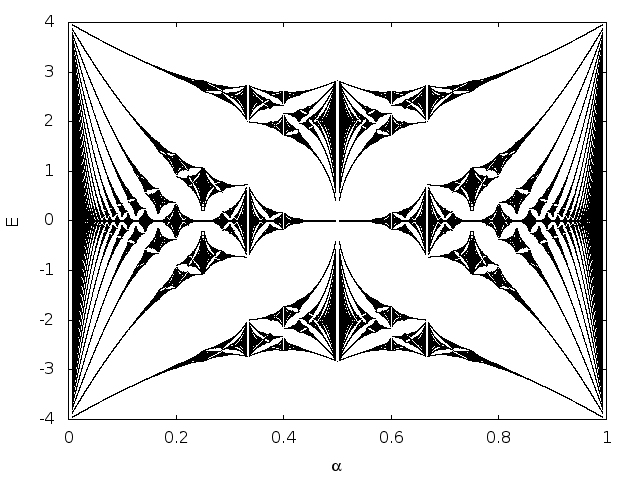
\includegraphics{butterfly}
 \centering
\end{figure}

\section{Metal-Insulator phase transition}
The Aubry-Andre model exhibits a phase transition from localized to delocalized behaviour at $\lambda = 2$ for Diophantine irrational numbers \cite{aulbach2004phase,aubry1980analyticity,jitomirskaya1999metal}. Localization means that the wavefunctions are concentrated at
certain lattice sites. Delocalized wavefunctions are roughly uniformly distributed at all lattice sites. Localized wavefunctions have insulator like properties with no effective
contribution to transport of charge, whereas the delocalized wavefunctions contribute to metallic behaviour. The quantitative measure of localization is called as the Inverse Participation Ratio (IPR).
It is defined as
\begin{equation}
 IPR = \frac{\sum_{n=1}^{L} |a_{n}|^4} {(\sum_{n=1}^{L} |a_{n}|^2)^2}
\end{equation} where $a_n$ are the expansion coefficients of the energy eigenstates in a local discrete-site basis and L is the number of lattice sites \cite{mishra2016phase, aulbach2004phase, aubry1980analyticity}.
IPR lies in the range $1$ to $1/L$, where $1$ indicates a perfectly localized state and $1/L$ indicates a perfectly delocalized state.

\begin{figure}[h]
\caption{ The metal-to-insulator transition of the
AAH Hamiltonian for the system’s ground state. Plot (a) shows the
IPR versus V0 or $\lambda$ in real space for L = 144, 1597 and 10 946 (top to
bottom) with $\alpha_0 = (\sqrt(5)-1)/2$ (inverse of golden ratio). The inset shows the variation of D2 with V0 which also
exhibits a transition. Plot (b) exhibits the mirror behavior in the dual
space}
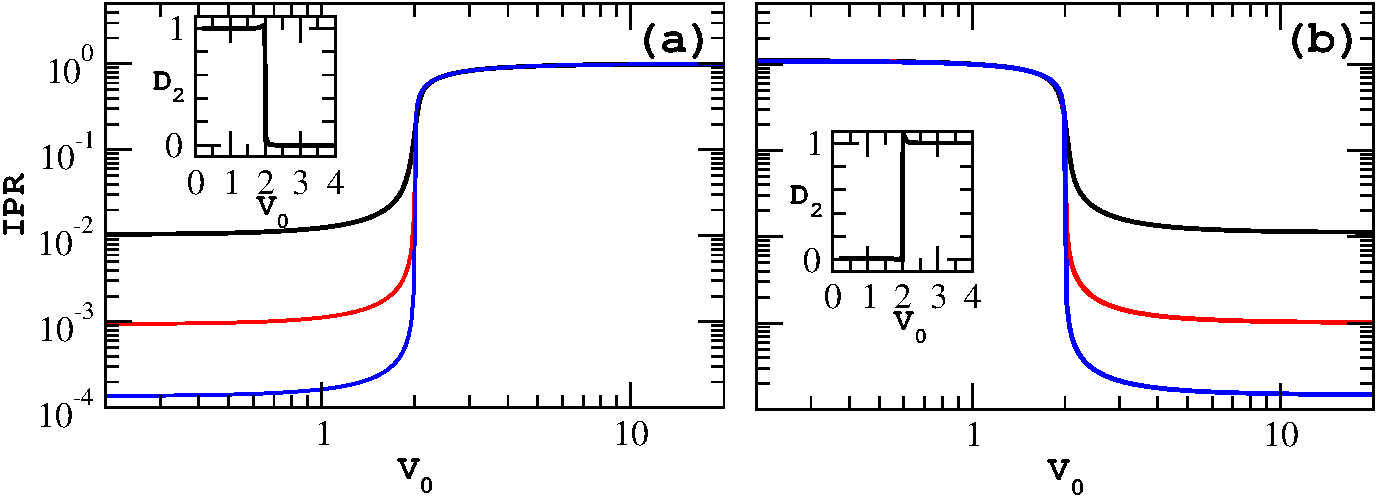
\includegraphics[width=0.75\textwidth]{AA-IPR-D2-Vs-V1byV2}
\centering
\end{figure}
AAH model has a duality transformation of the form \cite{aubry1980analyticity,aulbach2004phase,mishra2016phase}
\begin{equation}
 \ket{m} = \frac{1}{\sqrt{L}}\sum_{n}e^{-i2\pi\alpha_0 m n} \ket{n}
\end{equation} The effect of this transformation is to switch to a momentum space like representation. Wavefunctions localized in real space is delocalized in the dual space and vice versa.
AAH model is an exactly self-dual model i.e., the Hamiltonian retains its tri-diagonal form under the duality transformation, and the IPR plot in the dual space is an
exact mirror image of the IPR plot in the real space.
We also seek a relationship between IPR and $L$ of the form $IPR \propto L^{-D_2}$. The sharp transition of $D_2$ to 0 at $V_0 = 2$ indicates that this metal-insulator transition
is independent of length and true even under the limit of $L \rightarrow \infty$.

We shall use the IPR measure to evaluate the metal insulator phase transitions in the variants of the AAH model we study in this thesis.

\section{Hall Conductivity and Chern numbers}
As already mentioned in Chapter \ref{ch:qhe}, the Hall conductivity is a topological invariant. In fact, the harper model was  the first problem for which this result was established \cite{thouless1982quantized}. An interesting
discussion on chern numbers and their physical interpretation as applied to this problem can be found in \parencite{wen1989winding}. Another statement that chern numbers 
are the only topological invariants associated with energy bands is also shown using topological arguments \cite{avron1983homotopy}.
Hall conductivity can be calculated both numerically - using the Berry connection, and analytically - using the Streda formula.

Conductivity represents a linear relationship between the current density and the electric field. This is written as
\begin{equation}
 J_{i} = \sum_{j}\sigma_{ij}E_{j}
\end{equation} The off-diagonal term of the conductivity matrix is the hall conductivity.
\begin{equation}
 J_{i} = \sigma_{H}\epsilon_{ij}E_{j}
\end{equation} $\epsilon_{ij}$ is the levi-cevita symbol.
The local charge conservation of electromagnetism is represented by the continuity equation
\begin{equation}
 \mathbf{\nabla}\cdot\mathbf{J} = -\frac{\partial \rho}{\partial t}
\end{equation}
Therefore, for this problem we write
\begin{align}
 \frac{\partial \rho}{\partial t} &= -\mathbf{\nabla}\cdot\mathbf{J} \nonumber \\
 &= -(\partial_{x}J_{x} + \partial_{y}J_{y}) \nonumber \\
 &= -(\partial_{x}(\sigma_{h}E_{y}) + \partial_{y}(-\sigma_{h}E_{x})) \nonumber \\
 &= -\sigma_{H} (\partial_{x}E_{y} - \partial_{y}E_{x}) \nonumber  \\
 \text{Using Maxwell's equation}\\
 &= -\sigma_{H} \frac{\partial B}{\partial t} \nonumber \\
 \text{Therefore} \\
 \sigma_{H} &= \frac{\partial \rho}{\partial B}
\end{align}
This is known as the Streda formula \cite{streda1982quantised, bernevig2013topological}. $\rho$ used in the above equation is the charge density.
If the magnetic flux through an unit cell is a rational number $p/q$, then the charge density can be expressed in terms of
numbers of filled bands (bands below the fermi energy) $r$, as $e\frac{1}{V}\frac{r}{q}$ \cite{kohmoto1992flux,bernevig2013topological}, $V$ is the unit cell area.
Any three integers $p$, $q$ and $r$ can be related by the diophantine equation as
\begin{equation*}
 r = qs_{r} + pt_{r}
\end{equation*} where $s_{r},t_{r} \in \mathbb{Z}$ and $|t_{r}| \leq q/2$, $0\leq r \leq q$.
Implies that
\begin{equation*}
 \frac{r}{q} = s_{r} + \frac{p}{q}t_{r} = s_{r} + \frac{e}{h}BV t_{r}
\end{equation*} Therefore the Hall conductance when fermi level is in the rth gap is \footnote{Admittedly, this proof is not rigorous. Refer to \parencite{streda1982theory} for
a discussion in terms of Landau levels. Also, the TKNN paper also has a different way to arrive at the diophantine equation \cite{thouless1982quantized}.}
\begin{equation*}
 \sigma_{H} = \frac{e^2}{h}t_{r}
\end{equation*}

The Hall conductivity can be calculated numerically by simply performing the integral of the Berry curvature over the Brillouin zone torus. This is conveniently done using
the four-point Bargmann invariant formulation discussed in Chapter \ref{ch:gp}. The validity of this approach for discretized Brillouin zone has been established using 
lattice gauge theory \cite{fukui2005chern,hatsugai2006topological,aidelsburger2016artificial,rasta2016geometry}. The algorithm for the non-abelian case (works even in the presence of degeneracies) is presented step by step below. We intend to calculate chern number
for the $r$th gap.
\begin{enumerate}
 \item Write the Hamiltonian as a periodic function of $k_x$ and $k_y$. This was achieved in the previous section.
 \item Discretize the Brillouin zone. The discrete values of $k_x$ and $k_y$ are given by $k_x[j] = \frac{2\pi}{qN_{x}} j$ where $j=0,1\dots N_{x}-1$ and $k_y[j] = \frac{2\pi}{N_{y}} j$ where $j=0,1\dots N_{y}-1$. Roughly choose $N_{y} \sim qN_{x}$ \footnote{Using Landau gauge. However, this method is applicable for all gauge choices. Suitable modifications are required for symmetric gauge.}. 
 \item For each point on the discrete Brillouin zone, diagonalize the Hamiltonian. $\psi[k,i,j]$ denotes the $k$th eigenvector (eigenvectors ordered in ascending order of corresponding eigenvalues) of
 Hamiltonian at $k_x[i]$ and $k_y[j]$.
 \item For each point $(i,j)$ on the lattice, calculate $r \times r$ matrices $\mathbf{U}^{x}$ and $\mathbf{U}^{y}$. $U^{x}_{[a,b]} = \braket{\psi[a,i,j]|\psi[b,(i+1)mod\,N_{x},j]}$ and $U^{y}_[a,b] = \braket{\psi[a,i,j]|\psi[b,i,(j+1)mod\,N_{y}]}$, where $1\leq a,b \leq r$.
 We denote the $U_{x}[i,j] = \det(\mathbf{U}^{x})$ and $U_{y}[i,j] = \det(\mathbf{U}^{y})$.
 \item The four-point Bargmann invariant (equivalently the Berry curvature times the area) is calculated for each point as 
 \begin{equation*}
  F[i,j] = U_{x}[i,j]U_{y}[(i+1)mod\,N_{x},j]U_{x}^{*}[(i+1)mod\,N_{x},(j+1)mod\,N_{y}]U_{y}^{*}[i,(j+1)mod\,N_{y}]
 \end{equation*}
 \item The chern number is then calculated by summing up the Berry curvature values $C = \frac{1}{2\pi i}\sum_{i,j}F[i,j]$. 
\end{enumerate}
The chern numbers for the Harper-Hofstadter problem were successfully calculated using this method. Both methods, of course give the same results!

\begin{figure}[h]
 \centering
 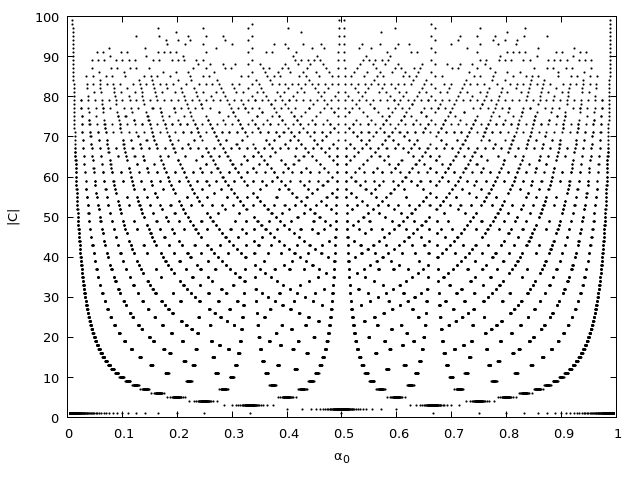
\includegraphics[width=\textwidth]{chern}
 \caption{Absolute value of Chern number $|C|$ of the lowest energy eigenstate as a function of magnetic flux $\alpha_0$.}
\end{figure}

  \part{Study of driven AAH models}
  % Author	Rajath Shashidhara
% Email		rajath.shashidhara@gmail.com
%
% This work is licensed under the Creative Commons Attribution 4.0 International License. 
% To view a copy of this license, visit http://creativecommons.org/licenses/by/4.0/.

\chapter{AAH model with Oscillating Magnetic Field}
Driving in this model is introduced in the form of a rapidly oscillating magnetic field perpendicular to the 2D lattice plane. This is a notoriously hard
problem because as magnetic flux varies with time, the $q$-subband structure is no longer present. In fact, $q$ is an extremely discontinuous function of time and of course
it cannot be ascribed a closed form description. This variant of the AAH model was absent in scientific literature until our recent publication \cite{mishra2016phase}.
We deal with this problem using the time-independent effective Hamiltonian picture presented in Chapter \ref{ch:fl}.

\section{Effective Hamiltonian}
Magnetic vector potential $\mathbf{A}(t)$ (written in Landau gauge) is
\begin{equation}
 \mathbf{A}(t) = Bx \cos(\omega t) \hat{\mathbf{y}}
\end{equation} where $\omega$ is the driving frequency, and it is assumed to be very high.
The Hamiltonian in the tight-binding form is
\begin{equation}
 \hat{H} = \sum_{n} \ket{n}\bra{n+1} + \ket{n}\bra{n-1} + V_{0}\cos(2\pi\alpha_{0}n\cos(\omega t) + \theta)\ket{n}\bra{n}
\end{equation}

The effective Hamiltonian up to order $\mathcal{O}(\frac{1}{\omega^3})$ is
\begin{equation}
 \begin{split}
  \hat{H}_{eff} &= \sum_{n} \ket{n}\bra{n+1} + \ket{n}\bra{n-1} + V_{0}\cos(\theta)\sum_{n}\mathcal{J}_{0}(2\pi\alpha_0 n)\ket{n}\bra{n} \\
  &- \frac{1}{2\omega^2}V_{0}^2 \cos^{2}(\theta) \sum_{n}\sum_{j=1} (\mathcal{J}_{2j}(2\pi\alpha_0 (n+1)) - \mathcal{J}_{2j}(2\pi\alpha_0 n))^2 \ket{n}\bra{n+1} \\
  &- \frac{1}{2\omega^2}V_{0}^2 \sin^{2}(\theta) \sum_{n}\sum_{j=1} (\mathcal{J}_{2j-1}(2\pi\alpha_0 (n+1)) - \mathcal{J}_{2j-1}(2\pi\alpha_0 n))^2 \ket{n}\bra{n+1} \\ 
  & + h.c.
 \end{split}
\end{equation}
Effective Hamiltonian is found to have retained the tri-diagonal structure in position space.

\section{Metal-Insulator transition}
This model also displays a sharp metal-insulator transition like the AAH model. However, it is not self-dual. A detailed discussion can be found
in \cite{mishra2016phase}.

\begin{figure}[h]
 \caption{The metal-to-insulator transition of the Effective Hamiltonian for the system’s ground state.  Plots (c) and (d) are the real- and dual-space plots for the
ground state with phase $\theta = 0$.}
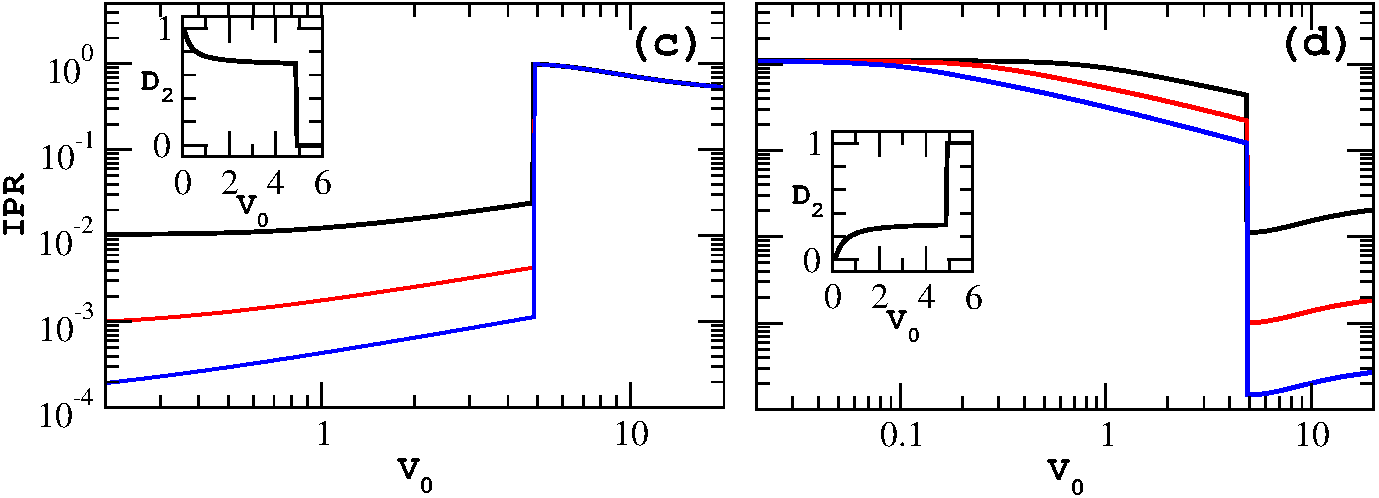
\includegraphics[width=0.85\textwidth]{FAA-Phase0-IPR-D2-Vs-V1byV2}
\centering
\end{figure}

\section{Spectrum}
The striking feature of the spectrum is the presence of energy-dependent mobility edge, an edge that splits the spectrum into two regions, one containing localized states and 
other containing delocalized states. This is a significant result as the mobility edge is atypical of 1-dimensional models \cite{mishra2016phase}.

\begin{figure}[ht]
\centering
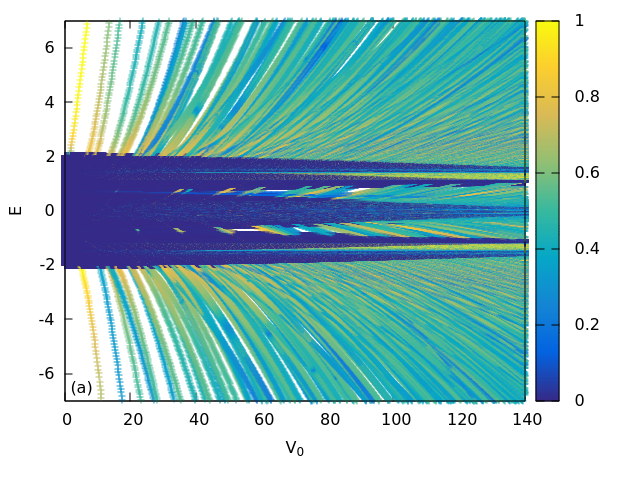
\includegraphics[width=0.65\textwidth]{evipr-4181-0.png}\\
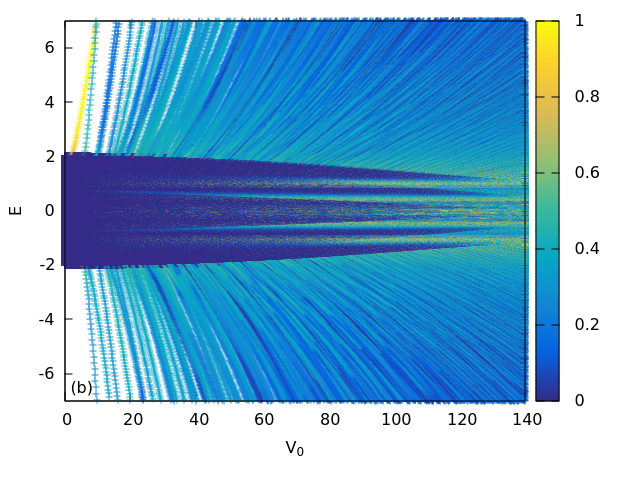
\includegraphics[width=0.65\textwidth]{evipr-4181-pi4.png}\\
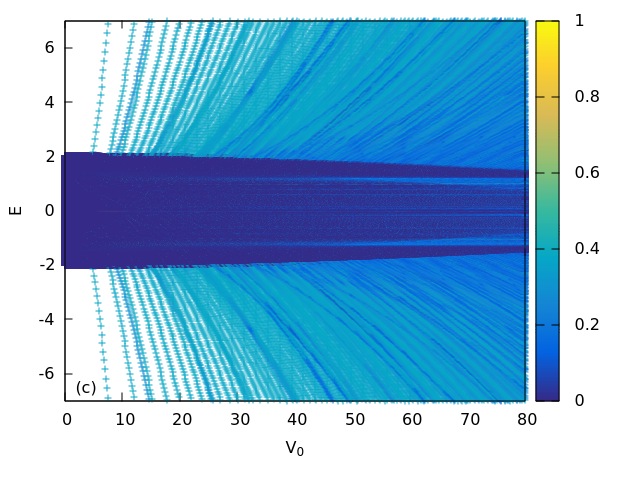
\includegraphics[width=0.65\textwidth]{evipr-4181-pi2.png}
\caption{The localization phase diagram with IPR in the (E,$V_0$) phase plane, for lattice size L = 4181 and three values of the variable $\theta$:
(a) $\theta = 0$, (b) $\theta = \pi/4$, (c) $\theta = \pi/2$}
\label{fig:mobedge}
\end{figure}

In order to qualitatively analyze some of our results we  consider a simplified model comprising of a trivial constant hopping term and an on-site potential $T$ which is aperiodic or quasi-periodic. The Schr\"odinger equation is given by  
\begin{equation}
\label{eq:AA}
 a_{n+1} + a_{n-1} + \Lambda  T(\alpha_0 n + \phi)a_n= Ea_n
\end{equation}
where,  $\Lambda$ is the strength of
on-site energy and $E$ are  the energy eigenvalues. One can go to the dual
space for the above system by defining an expansion, as follows
\begin{equation}
\label{trans1}
 a_n = \frac{ e^{ikn}}{\sqrt L}\displaystyle\sum_m \tilde{a}_m
 e^{i\,m(\alpha_0 n + \phi)}
\end{equation}
where, the $\tilde{a}_m$'s are the dual space amplitudes, and $k$ is a wave vector
from the Bloch wave expansion ansatz.  This  allows 
 $T$  to be expressed as
\begin{equation}
\label{trans2}
  T(\alpha_0 n+ \phi) = \frac{1}{\sqrt L}\displaystyle\sum_{\acute{m}}\mathcal{T}_{\acute{m}} e^{i\,\acute{m}(\alpha_0 n + \phi)}.
\end{equation}

Equations \eqref{trans1} and \eqref{trans2}  yield an on-site term in the dual space from the the hopping terms of Eq.\eqref{eq:AA} as  
\begin{equation}
\label{eq:Fspacesite}
a_{n-1} + a_{n+1} = \frac{e^{ikn}}{\sqrt L}\displaystyle\sum_m \tilde{a}_m e^{i\,m(\alpha_0 n + \phi)} \cos(\alpha_0 m + k)
\end{equation}
with a cosine modulation of the on-site energy  (as seen in
the Aubry and Andr\'e model). Interestingly, the real space on-site energy term transforms as
\begin{equation}
\Lambda  T(\alpha_0 n + \phi)a_n= \frac{\Lambda e^{ikn}}{L}\displaystyle\sum_{\acute{m}}\displaystyle\sum_m\mathcal{T}_{\acute{m}}\tilde{a}_m e^{i\,(m + \acute{m})(\alpha_0 n+\phi)}.   
\end{equation}
The RHS can be slightly rearranged to give 
\begin{equation}
\label{farTB}
\begin{split}
\frac{\Lambda e^{ikn}}{L}&\displaystyle\sum_{\acute{m}\neq\pm1}\displaystyle\sum_m\mathcal{T}_{\acute{m}}\tilde{a}_{m + \acute{m}} e^{i\,m(\alpha_0 n+\phi)} +\\ 
& \frac{\Lambda e^{ikn}}{L}\displaystyle\sum_m (\mathcal{T}_1\tilde{a}_{m-1} + \mathcal{T}_{-1}\tilde{a}_{m+1})e^{i\,m(\alpha_0 n + \phi)} 
\end{split}
\end{equation}
In the above form,  the second term clearly indicates the apparent nearest
neighbor hopping terms in the dual space whose strength is modulated
by the Fourier components of $T$. It is the first term in the above
expression which explicitly breaks the exact duality. The form of
$\mathcal{T}_{\acute{m}}$ determines the extent to which different
$m$ values in the dual space are coupled.  It is well known
that for decaying oscillatory functions like Sinc and Bessel function
of the zeroth order $\mathcal{T}_{\acute{m}}$ is a rectangular
function,   with possibly a $\acute{m}$ dependent modulation,  symmetric
about the origin. Thus,  in our case, we expect a truncation effect in
dual space which restricts the range of couplings. This deviation from
exact duality is expected to have some impact on the
probability of an ``analytic accident'' along the lines of \parencite{aubry1980analyticity}.
The appearance of localized states (real eigenfunctions) happens when
there are superpositions of counter-propagating plane waves with
wave vectors of near-commensurate magnitude. This would mean,  in our
model, some harmonics from the expansion of $T$ shall scatter the wave with
wave vector $k$ by an amount commensurate with $2n\pi$. This has to be
considered together with the fact that for a rational approximation of
$\alpha_0$ as a ratio of two large successive Fibonacci numbers, the
true momentum(Fourier) space eigenvalues $\kappa$ are related to $m$
as $ \kappa = mF_{i-1}\textrm{mod}F_i$, where $F_{i-1}$ and $F_i$ are
successive Fibonacci numbers \parencite{kohmoto1983metal,aulbach2004phase}. Thus, what appear
to be close neighbors in $m$ could possibly be well separated in the
actual wave vector space. Further, the range of $m$ values that shall
remain coupled in the dual space will be dictated by the extent of
$T$ in the real lattice for example the first zero in the Bessel
function. The set of $m$'s which conspires with a given $k$ value to
yield a localized state shall be dictated by $V_0$ and $E(k)$. This
explains the energy dependent mobility edge in Fig.\ref{fig:mobedge}. 

In the dual space, where $k$ acts as a phase (see Eq.\eqref{eq:Fspacesite}), a
state localized at few $m$ values could be  shifted by large amounts
for a small change in $k$. This allows for the interpretation that a
small change in $\phi$ could in effect cause a state localized around
some lattice site to localize about a far off site.
 In terms of symmetry, the absence of 
translational invariance in Euclidean space of quasi-periodic
structures with two incommensurate periodicities can be restored in an
extended space using the $\phi$ dimension \cite{sokoloff1985unusual, janner1977symmetry}. This
effect of $\phi$ on localization properties leads to the differences between the
three plots in Fig.\ref{fig:mobedge}.  

  % Author	Rajath Shashidhara
% Email		rajath.shashidhara@gmail.com
%
% This work is licensed under the Creative Commons Attribution 4.0 International License. 
% To view a copy of this license, visit http://creativecommons.org/licenses/by/4.0/.

\chapter{AAH model driven by Linearly Polarized Light}
We drive the AAH system by an electric field oriented along one of the lattice vector directions. The motivation for such a model is that it presents a more accurate description
of the Quantum Hall effect. Magnetic field in the plane of the lattice does not affect the motion of electrons restricted to 2-dimensional lattice (from Lorentz's force law). Therefore,
this feature of linearly polarized light may be effectively ignored.

Adding an electric field that is constant across the space does not change the periodicity properties of the Hamiltonian. The magnetic translation vectors are multiplied by a
constant phase factor and the magnetic translation group can be defined on the same lines as the pure AAH case. Correspondingly, the q-subband structure is not affected by this driving.

The magnetic vector potential corresponding to the system is
\begin{equation}
 \mathbf{A}(t) = (Bx + A\cos(\omega t)) \hat{\mathbf{y}}
\end{equation}
Using Peirels substitution as shown in Chapter \ref{ch:aah}, the Hamiltonian in the tight-binding form can be obtained.
\section{Effective Hamiltonian}
Following the same presciption detailed in Chapter \ref{ch:aah}, the Hamiltonian in real space is represented by the recursive equation
\begin{equation}
 a_{n+1} + a_{n-1} + 2\lambda\cos(2\pi(\alpha_0 + \alpha \cos{\omega t}) + \theta) a_{n} = E a_{n}
\end{equation} where $\alpha_0 = \frac{e}{h}Bd^2$ and $\alpha = \frac{e}{h}Ad$.

To proceed further, we shall apply the Floquet-BW perturbation theory to obtain the time-independent effective Hamiltonian.
Using the trignometric results listed in Appendix \ref{app:trig}, the fourier components of the Hamiltonian are
\begin{equation}
 H^{m,n}_{i,j} = \begin{cases}
            \delta_{i+1,j} + \delta_{i,j+1} + 2\lambda \mathcal{J}_{0}(2\pi\alpha) \cos(\theta + 2\pi\alpha_0 j) \;\delta_{i,j} & m=n\\
            (-1)^{\frac{|m-n|}{2}} \;2\lambda \mathcal{J}_{|m-n|}(2\pi\alpha) \cos(\theta + 2\pi\alpha_0 j) \;\delta_{i,j} & |m-n| \text{ is even}\\
            (-1)^{\frac{|m-n|+1}{2}} \;2\lambda \mathcal{J}_{|m-n|}(2\pi\alpha) \sin(\theta + 2\pi\alpha_0 j) \;\delta_{i,j} & |m-n| \text{ is odd}
           \end{cases}
\end{equation}
$H_{BW}^{(1)}$  is zero because
\begin{equation*}
 \frac{H_{0,n}H_{n,0}}{n\omega} + \frac{H_{0,-n}H_{-n,0}}{(-n)\omega} = 0
\end{equation*}
$H_{BW}^{(2)}$ only contributes to diagonal terms because of the structure of fourier components detailed above.

The momentum space Hamiltonian for this problem can be derived using the same approach used in the pure AAH case.
\begin{equation}
 H(k_x, k_y, t)_{i,j} = \delta_{i+1,j} + \delta_{i,j+1} + 2\lambda\cos(k_y + 2\pi\alpha_0 j - 2\pi\alpha \cos{\omega t}) \delta_{i,j} + e^{-iqk_x} \delta_{i,1}\delta_{j,q} + e^{iqk_x} \delta_{i,q}\delta_{j,1}
\end{equation} where $k_x \in [-\pi/q, \pi/q]$, $k_y \in [-\pi,\pi]$ and $i,j \in 1\dots q$.
Consequently, the fourier components are
\begin{equation}
 H^{m,n}_{i,j}(k_x, k_y) = \begin{cases}
            \begin{split}\delta_{i+1,j} + \delta_{i,j+1} + e^{-iqk_x} \delta_{i,1}\delta_{j,q} + e^{iqk_x} \delta_{i,q}\delta_{j,1} \\+ 2\lambda \mathcal{J}_{0}(2\pi\alpha) \cos(\theta + 2\pi\alpha_0 j) \;\delta_{i,j}\end{split} & m=n\\
            (-1)^{\frac{|m-n|}{2}} \;2\lambda \mathcal{J}_{|m-n|}(2\pi\alpha) \cos(\theta + 2\pi\alpha_0 j) \;\delta_{i,j} & |m-n| \text{ is even}\\
            (-1)^{\frac{|m-n|-1}{2}} \;2\lambda \mathcal{J}_{|m-n|}(2\pi\alpha) \sin(\theta + 2\pi\alpha_0 j) \;\delta_{i,j} & |m-n| \text{ is odd}
           \end{cases}
\end{equation}
$H_{BW}$ is numerically computed from the above fourier components up to order $\mathcal{O}(1/\omega^3)$.
\section{Results}
We shall analyze the perturbation terms arising due to the linear electric field. The perturbation terms contribute to each lattice site uniformly i.e., they are independent of
the lattice site index. Further, they only affect the on-site terms. On-site terms are akin to potential energy assigned to each lattice site and off-site terms are hopping terms,
and they are indicators of kinetic energy due to hopping of electrons between neighbors in the lattice.

\begin{figure}[t]
 \centering
 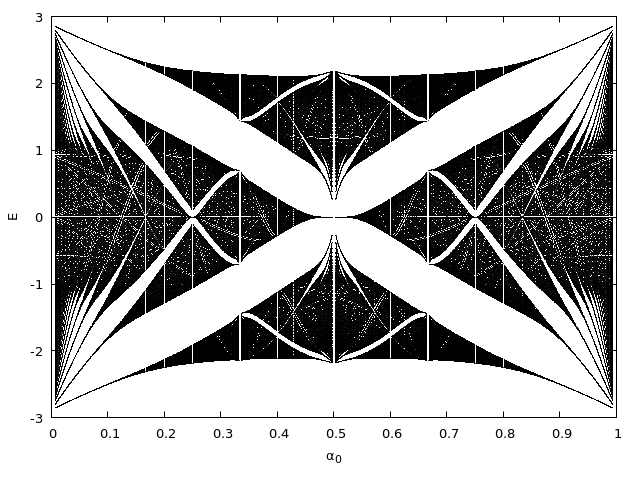
\includegraphics[width=0.65\textwidth]{linear-spectrum}\\
 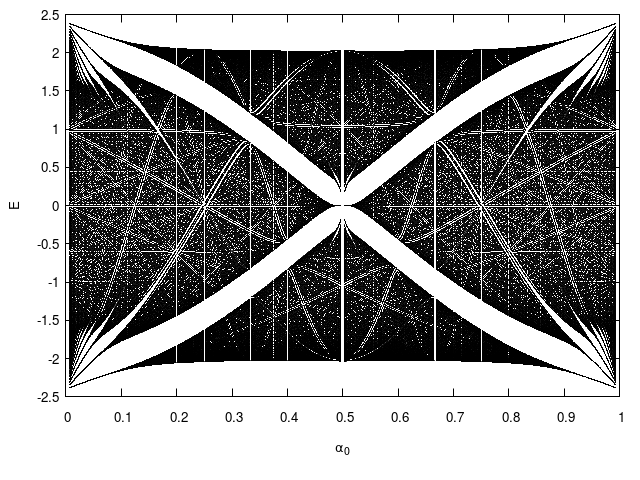
\includegraphics[width=0.65\textwidth]{linear-spectrum5}\\
 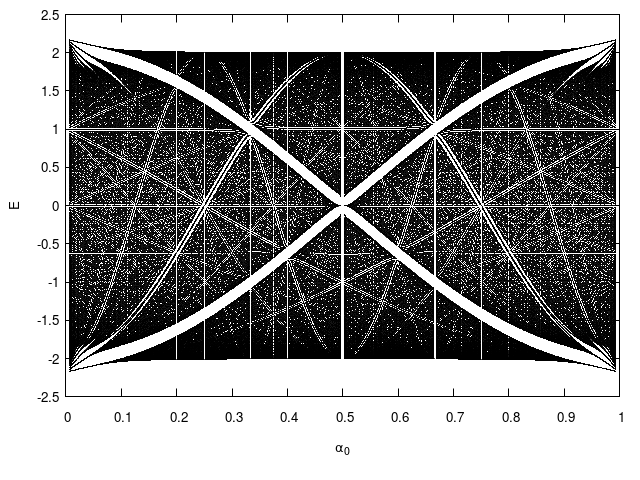
\includegraphics[width=0.65\textwidth]{linear-spectrum25}
 \caption{Spectrum of the driven Aubry-Andr\'e-Harper model by linearly polarized electric field. The parameters are set to $\lambda=1.0$, $\omega=1.0$ and $k_x=0, k_y=0$.
 (a) $\alpha = 1.0$ (b) $\alpha = 5.0$ (c) $\alpha = 25.0$}
\end{figure}

As the magnitude of electric field increases, the range of energy eigenvalues is diminishing and the gaps in the spectrum are compacted. The same effect can be achieved by increasing
the $\lambda$ in the pure AAH model. However, the perturbation terms include products of $\cos(\theta + 2\pi\alpha_0 j)$ and $\sin(\theta + 2\pi\alpha_0 j)$ accompanied by
oscillatory multiplicative factors in the form of bessel functions, to the on-site terms. It is nearly impossible to gauge the impact of the perturbation terms on
the recursive structure of the graph. Analysis of this nature requires mathematical skills beyond the abilities of the author at the time of writing this document.

We examine the nature of metal-insulator transition for ground state of real-space Hamiltonian using the plot of $IPR$ vs. $\lambda$ and $IPR$ vs. $\alpha$.
\begin{figure}[h]
 \centering
 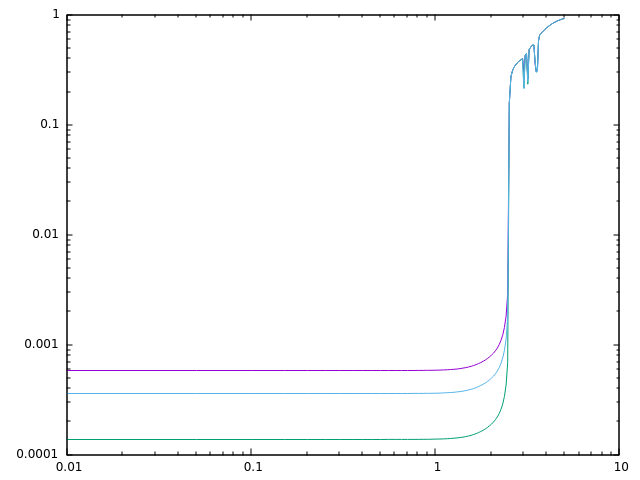
\includegraphics[width=0.45\textwidth]{ipr-linear}
 \caption{Plot of $IPR$ vs $\lambda$ for $L=2584,4181,10946$ and  $\alpha=1.0, \alpha_0=1/goldenratio$.}
\end{figure}

When the chern numbers are plotted against $\alpha$, the topological transitions are unveiled. This discovery is quite intriguing as the transitions are periodic and they seem to
be independent of $\alpha_0$. Also, the width of transition is increasing as $\alpha$ increases. A deeper analysis of undergoing phenomenon must be carried out to understand the 
observations. This reported is limited to calculation of chern numbers. Analysis will be published in a future work.

The relationship between Chern numbers and Hall conductivity for time-dependent systems is non-trivial and requires further literature survey to understand it. This has not been 
taken up as a part of this thesis. However, a transition in chern number clearly indicates a topological transition and this in some way impacts the physical quantities.
\begin{figure}[h]
 \centering
 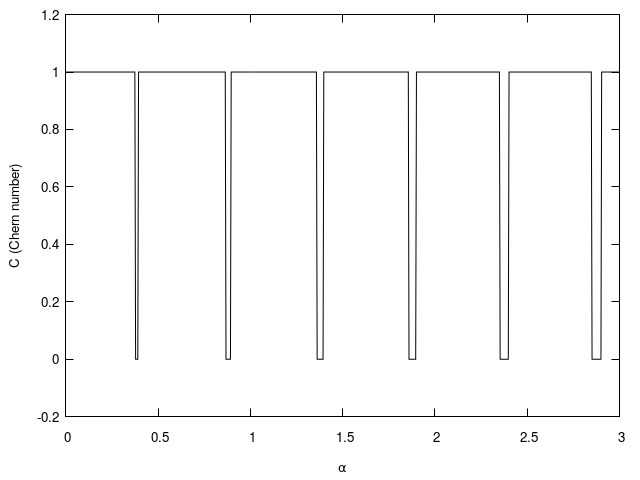
\includegraphics[width=0.45\textwidth]{linear-chern-3a}\\
 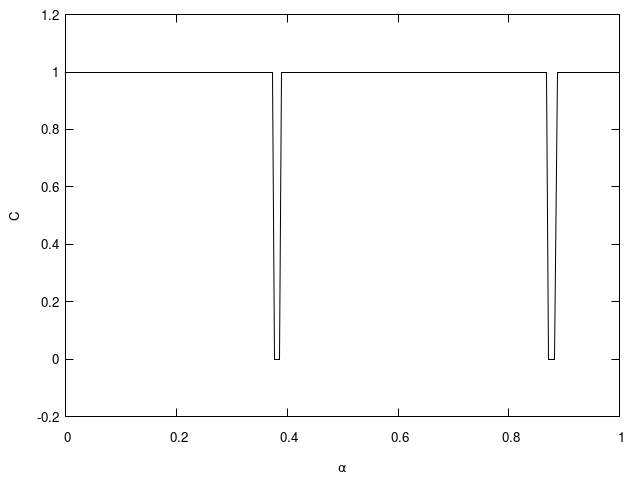
\includegraphics[width=0.45\textwidth]{linear-chern-5a}
 \caption{Plot of Chern numbers of the lowest subband vs. $\alpha$ for (a) $\alpha_0 = 1/3$ (b) $\alpha_0 = 1/5$.}
\end{figure}

  % Author	Rajath Shashidhara
% Email		rajath.shashidhara@gmail.com
%
% This work is licensed under the Creative Commons Attribution 4.0 International License. 
% To view a copy of this license, visit http://creativecommons.org/licenses/by/4.0/.

\chapter{AAH model driven by Circularly Polarized Light}
%   % Author	Rajath Shashidhara
% Email		rajath.shashidhara@gmail.com
%
% This work is licensed under the Creative Commons Attribution 4.0 International License. 
% To view a copy of this license, visit http://creativecommons.org/licenses/by/4.0/.

\chapter{AAH model with oscillatory hopping potential}

    
  \renewcommand{\thechapter}{\Alph{chapter}}
  \part{Appendices}
    \chapter{Effective Hamiltonian - perturbative expansion}\footnote{This chapter was wholly borrowed from Tridev Mishra, Ph.D Student, Department of Physics, BITS Pilani. (\url{tridevmishra@gmail.com})}
As derived in Chapter \ref{ch:fl}, we are looking to perturbatively expand the equation
\begin{equation}
 \label{app_da:unitary}\hat{H}_{eff}= e^{i\hat{F}(t)}\hat{H}e^{-i\hat{F}(t)} + i\frac{\partial}{\partial t}\left(e^{i\hat{F}(t)}\right)e^{-i\hat{F}(t)}
\end{equation}

The entire solution is divided into 
 \begin{enumerate}
  \item Initial Kick $(e^{i\hat{F}(t_{i})})$
  
  \item Evolution under a time-independent Hamiltonian $\hat{H}_{eff} (e^{-i\hat{H}_{eff}(t_{f}-t{i})})$
  
  \item Final Kick $(e^{-i\hat{F}(t_{i})})$
 \end{enumerate}
 Consider periodic potentials
 \begin{equation*}
  \hat{V}(t) = \hat{V}(t+T)
 \end{equation*}
 assume $T$ to be small and $\omega = \frac{2\pi}{T}$ to be large. Except for special cases $\hat{H}_{eff}$ cannot be obtained 
 from $(5)$ in a closed form.
 
 Let us make a perturbation ansatz.
 \begin{gather}
   \hat{H}_{eff}=\displaystyle\sum_{0\leq n< \infty}\frac{1}{\omega^{n}}\hat{H}^{(n)} \\
   \hat{F}= \displaystyle\sum_{1\leq n< \infty}\frac{1}{\omega^{n}}\hat{F}^{(n)}
 \end{gather} 
 Convergence is not guaranteed.
 
 The prescription is
%  \renewcommand{\theenumi}{\alph{enumi}}
 \begin{enumerate}
  \item Write Eqn. \eqref{app_da:unitary} for $\hat{H}_{eff}$ as an expanded perturbation series in $(\frac{1}{\omega})$.
  
  \item At each order of perturbation, which corresponds to a specific power of $(\frac{1}{\omega})$ retain the time-independent
  average in $\hat{H}_{eff}$ and adjust $\hat{F}$ to annhilate any time dependence.
  
  \item Repeat the procedure at each order in perturbation.
 \end{enumerate}

 We use the following identities: 
 \begin{gather}
  e^{i\hat{F}}\hat{H}e^{-i\hat{F}}= \hat{H} + i[\hat{F},\hat{H}] -\frac{1}{2}\left[\hat{F},[\hat{F}'\hat{H}]\right]-\frac{i}{6}\Biggl[\hat{F},\left[\hat{F},[\hat{F},\hat{H}]\right]\Biggr]+\dots \\
  \left(\frac{\partial}{\partial t}e^{\hat{F}}\right)e^{-i\hat{F}}= i\frac{\partial\hat{F}}{\partial t}-\frac{1}{2}[\hat{F},\frac{\partial\hat{F}}{\partial t}]-\frac{i}{6}\left[\hat{F},[\hat{F},\frac{\partial\hat{F}}{\partial t}]\right]+\dots
 \end{gather}
 
 Substituting $\hat{H}_{eff} =\displaystyle\sum_{0\leq n< \infty}\frac{1}{\omega^{n}}\hat{H}^{(n)}$ and 
 $\hat{F}= \displaystyle\sum_{1\leq n< \infty}\frac{1}{\omega^{n}}\hat{F}^{(n)}$ in Eqn. \eqref{app_da:unitary} and only retaining upto $\mathcal{O}\left(\frac{1}{\omega^2}\right)$
 we have
 
 \begin{eqnarray*}
 \begin{split}
  \hat{H}_{eff}= \hat{H}_{o}+ \hat{V}(t) +
  i\left[\frac{\hat{F}^{(1)}}{\omega},\hat{H}\right]+i\left[\frac{\hat{F}^{(2)}}{\omega^2},\hat{H}\right]   
  -\frac{1}{2}\Biggl[\frac{\hat{F}^{(1)}}{\omega},\left[\frac{\hat{F}^{(1)}}{\omega},\hat{H}\right]\Biggr]-\frac{1}{\omega}\frac{\partial\hat{F}^{(1)}}{\partial
    t} - \frac{1}{\omega^2}\frac{\partial\hat{F}^{(2)}}{\partial
    t}\\    -\frac{1}{\omega^3}\frac{\partial\hat{F}^{(2)}}{\partial t} 
  -\frac{i}{2}\left[\frac{\hat{F}^{(1)}}{\omega}+\frac{\hat{F}^{(2)}}{\omega^2},\frac{1}{\omega}\frac{\partial\hat{F}^{(1)}}{\partial
      t}+ \frac{1}{\omega^2}\frac{\partial\hat{F}^{(2)}}{\partial
      t}\right] +
  \frac{1}{6}\Biggl[\frac{\hat{F}^{(1)}}{\omega},\left[\frac{\hat{F}^{(1)}}{\omega},\frac{1}{\omega}\frac{\partial\hat{F}^{(1)}}{\partial
        t}\right]\Biggr]
 \end{split}
\end{eqnarray*}\par

The operator $\hat{F}$ is periodic with period $T$ and has zero mean.
\begin{equation*} 
  \Rightarrow\frac{1}{T}\int\limits_{0}^{T}\hat{F}dt=0
\end{equation*}
$\Rightarrow \hat{F}^{(n)}$ are all periodic and have zero mean or 
\begin{gather*}
  \langle \hat{F}^{(n)} \rangle=0 \\
  \hat{F}^{(n)}(t+T)=\hat{F}^{(n)}(t)
\end{gather*}

At each order in perturbation, the time independent average is retained in $\hat{H}_{eff}$ and
$\hat{F}$ is used to nullify the time dependent part.

ORDER $\omega^0$ :
\begin{equation*}
 \hat{H}_{0}+\hat{V}(t)-\frac{1}{\omega}\frac{\partial\hat{F}^{(1)}}{\partial t}
\end{equation*}
\begin{align*}
 H^{(0)}_{eff} &= \left\langle \hat{H}_0+ \hat{V}(t)-\frac{1}{\omega}\frac{\partial\hat{F}^{(1)}}{\partial t}\right\rangle \\
 &= \langle\hat{H}_0\rangle+ \langle\hat{V}(t)\rangle -\frac{1}{\omega}\left\langle\frac{\partial\hat{F}^{(1)}}{\partial t}\right\rangle \\
 &= \frac{\hat{H}_{0}}{T}\int\limits_{0}^{T}dt + \frac{1}{T}\int\limits_{0}^{T}\hat{V}(t)dt -\frac{1}{\omega T}\int\limits_{0}^{T}\frac{\partial\hat{F}^{(1)}}{\partial t}dt 
\end{align*}
\begin{equation*}
  \hat{V}(t)= \hat{V}(t+T)
\end{equation*}
$ \hat{V}(t)$ may be expanded in a Fourier series as 
\begin{equation*}
 \hat{V}(t)= \hat{V}_0 + \displaystyle\sum_{1\leq n<\infty}\hat{V}_{n}e^{in\omega t} + \displaystyle\sum_{1\leq n<\infty}\hat{V}_{-n}e^{-in\omega t}
\end{equation*}
$\hat{F}^{(1)}$ can be expanded similarly but $\hat{F}^{(1)}$ has zero mean. So $\frac{\partial\hat{F}^{(1)}}{\partial t}$ also has zero mean.
\begin{equation*}
 H_{eff}^{(0)} = \hat{H}_0 + \hat{V}_0 ~~~~~~~~ \hat{V}_0 = \frac{1}{T}\int\limits_{0\leq t\leq T}\hat{V}(t)dt
\end{equation*}
The time dependent part is 
~~~~~~~~~$$ \hat{H}_{0}+\hat{V}(t)-\frac{1}{\omega}\frac{\partial\hat{F}^{(1)}}{\partial t} -\left\langle \hat{H}_0+ \hat{V}(t)-\frac{1}{\omega}\frac{\partial\hat{F}^{(1)}}{\partial t}\right\rangle$$

~~~~~~~$$\Rightarrow \hat{V}(t) -\hat{V}_0 -\frac{1}{\omega}\frac{\partial\hat{F}^{(1)}}{\partial t}$$(equating this to zero)

or ~~~~~~~$$\displaystyle\sum_{1\leq n<\infty}\hat{V}_{n}e^{in\omega t} + \displaystyle\sum_{1\leq n<\infty}\hat{V}_{-n}e^{-in\omega t} = \frac{1}{\omega}\frac{\partial\hat{F}^{(1)}}{\partial t}$$

~~~~~~~$$\Rightarrow \hat{F}^{(1)} = \omega\int\limits_{0}^{t}\left(\displaystyle\sum_{1\leq n<\infty}\hat{V}_{n}e^{in\omega \acute{t}} + \displaystyle\sum_{1\leq n<\infty}\hat{V}_{-n}e^{-in\omega \acute{t}}\right)d\acute{t}$$

~~~~~~~$$\Rightarrow \frac{1}{i}\displaystyle\sum_{1\leq n<\infty}\frac{1}{n}\biggl(\hat{V}_{n}e^{in\omega t} -\hat{V}_{-n}e^{-in\omega t}\biggr)$$

or ~~~~~ at order $\omega_0$

~~~~~~~~~$$H_{eff}^{(0)} = \hat{H}_{0} + \hat{V}_0 $$

~~~~~~~~~$$\hat{F}^{(1)} = \frac{1}{i}\displaystyle\sum_{n}\frac{1}{n}\biggl(\hat{V}_{n}e^{in\omega t} -\hat{V}_{-n}e^{-in\omega t}\biggr)$$

ORDER $\omega^{-1}$

~~~~~~~~~$$i\left[\frac{\hat{F}^{(1)}}{\omega},\hat{H}\right]- \frac{1}{\omega^2}\frac{\partial\hat{F}^{(2)}}{\partial t}
 - \frac{i}{2}\left[\frac{\hat{F}^{(1)}}{\omega},\frac{1}{\omega}\frac{\partial \hat{F}^{(1)}}{\partial t}\right]$$
 
~~~~~~~~~$$H_{eff}^{(1)} = \left\langle i\biggl[\frac{\hat{F}^{(1)}}{\omega},\hat{H}\biggr]\right\rangle-\left\langle\frac{1}{\omega^2}\frac{\partial\hat{F}^{(2)}}{\partial t}\right\rangle
- \frac{i}{2}\left\langle\biggl[\frac{\hat{F}^{(1)}}{\omega},\frac{1}{\omega}\frac{\partial \hat{F}^{(1)}}{\partial t}\biggr]\right\rangle$$

The second bracket in the above expression is put to zero.Hence

~~~~~~~~~$$H_{eff}^{(1)} = i\left\langle \biggl[\frac{\hat{F}^{(1)}}{\omega},\hat{H}\biggr]\right\rangle- \frac{i}{2}\left\langle\biggl[\frac{\hat{F}^{(1)}}{\omega},\frac{1}{\omega}\frac{\partial \hat{F}^{(1)}}{\partial t}\biggr]\right\rangle$$

~~~~~~~~~~~$$= i\left\langle \biggl[\frac{\hat{F}^{(1)}}{\omega},(\hat{V}(t)-\hat{V}_0)\biggr]\right\rangle -\frac{i}{2}\left\langle\biggl[\frac{\hat{F}^{(1)}}{\omega},(\hat{V}(t)-\hat{V}_0)\biggr]\right\rangle$$

~~~~~~~~~~~$$=\frac{i}{2}\left\langle\biggl[\frac{\hat{F}^{(1)}}{\omega},(\hat{V}(t)-\hat{V}_0)\biggr]\right\rangle$$

$$\hat{V}(t)-\hat{V}_0 = \displaystyle\sum_{n}\frac{1}{n}\biggl(\hat{V}_{n}e^{in\omega t} -\displaystyle\sum_{n}\hat{V}_{-n}e^{-in\omega t}\biggr)$$

$$ \hat{F}^{(1)} = \int\limits_{}^{t}(\hat{V}(\acute{t})-\hat{V}_0)d\acute{t}$$

$$ \frac{\hat{F}^{(1)}}{\omega} = \displaystyle\sum_{n}\biggl(\frac{\hat{V}_{n}e^{in\omega t}}{in\omega}-\frac{\hat{V}_{-n}e^{-in\omega t}}{in\omega}\biggr)$$

$$ \left\langle \frac{\hat{F}^{(1)}}{\omega}(\hat{V}(t)-\hat{V}_{0})\right\rangle = \frac{1}{T}\int\limits_{0}^{t}\displaystyle\sum_{n,m}\biggl(\frac{\hat{V}_{n}e^{in\omega\acute{t}}}{in\omega}-\frac{\hat{V}_{-n}e^{-in\omega\acute{t}}}{in\omega}\biggr)
\biggl(\hat{V}_{m}e^{im\omega\acute{t}}+\hat{V}_{-m}e^{-im\omega\acute{t}}\biggr)$$

$$ = \frac{1}{T}\int\limits_{0}^{T}d\acute{t}\displaystyle\sum_{m,n}\frac{\hat{V}_n\hat{V}_m}{in\omega}e^{i(n+m)\omega\acute{t}}+ \frac{\hat{V}_n\hat{V}_{-m}}{in\omega}e^{i(n-m)\omega\acute{t}}
- \frac{\hat{V}_{-n}\hat{V}_m}{in\omega}e^{-i(n-m)\omega\acute{t}} - \frac{\hat{V}_{-n}\hat{V}_{-m}}{in\omega}e^{-i(n+m)\omega\acute{t}}$$

\begin{eqnarray}
 = \displaystyle\sum_{n}\frac{\hat{V}_n\hat{V}_{-n}}{in\omega} - \frac{\hat{V}_{-n}\hat{V}_n}{in\omega}
\end{eqnarray}

\begin{eqnarray}
 \left\langle(\hat{V}(t)-\hat{V}_0)\frac{\hat{F}^{(1)}}{\omega}\right\rangle = \displaystyle\sum_{n}\frac{\hat{V}_{-n}\hat{V}_{n}}{in\omega} - \frac{\hat{V}_{n}\hat{V}_{-n}}{in\omega} = \displaystyle\sum_{n}\frac{2}{in\omega}[\hat{V}_n,\hat{V}_{-n}]
\end{eqnarray}

% $(8) - (9)$
% 
% $$ \Rightarrow \displaystyle\sum_{n}\frac{2}{in\omega}[\hat{V}_n,\hat{V}_{-n}]$$

or $$ H_{eff} = \frac{i}{2}\displaystyle\sum_{n}\frac{2}{in\omega}[\hat{V}_n,\hat{V}_{-n}]$$

$$ = \displaystyle\sum_{n}\frac{1}{n\omega}[\hat{V}_n,\hat{V}_{-n}]$$

$$ i\biggl[\frac{\hat{F}^{(1)}}{\omega},\hat{H}\biggr]- \frac{1}{\omega^2}\frac{\partial\hat{F}^{(2)}}{\partial t}
 - \frac{i}{2}\biggl[\hat{F}^{(1)},\frac{\partial \hat{F}^{(1)}}{\partial t}\biggr]-\displaystyle\sum_{n}\frac{1}{n\omega}[\hat{V}_n,\hat{V}_{-n}]=0$$
 
 $$ \Rightarrow \hat{F}^{(2)} = \frac{1}{i}\displaystyle\sum_{n}\frac{1}{n^2}\biggl([\hat{V}_n,\hat{H}_0+\hat{V}_0]e^{in\omega t}-h.c.\biggr)
  + \frac{1}{2i}\displaystyle\sum_{n,m=1}^{\infty}\frac{1}{n(n+m)}\biggl([\hat{V}_n,\hat{V}_m]e^{i(n+m)\omega t} + h.c.\biggr)$$
 $$ + \frac{1}{2i}\displaystyle\sum_{n\neq m=1}^{\infty}\frac{1}{n(n+m)}\biggl([\hat{V}_n,\hat{V}_{-m}]e^{i(n-m)\omega t} + h.c.\biggr)$$
 
 Finally, we have in the same manner
 
 $$ \hat{H}_{eff} = \hat{H}_0 + \hat{V}_0+ \frac{1}{\omega}\displaystyle\sum_{n=1}^{\infty}\frac{1}{n}[\hat{V}_n,\hat{V}_{-n}] + \frac{1}{2\omega^2}
 \displaystyle\sum_{n=1}^{\infty}\frac{1}{n^2}\biggl(\biggl[[\hat{V}_n,\hat{H}_0],\hat{V}_{-n}\biggr]+h.c. \biggr)$$
 $$ +\frac{1}{3\omega^2}\displaystyle\sum_{n,m=1}^{\infty}\frac{1}{nm}\biggl(\biggl[\hat{V}_n,[\hat{V}_m,\hat{V}_{-(n+m)}]\biggr] -2\biggl[\hat{V}_n,[\hat{V}_{-n}
 ,\hat{V}_{(n-m)}]\biggr] + h.c.\biggr)$$
 
 and\\
 
 $$ \hat{F}(t)= \frac{1}{i\omega}\displaystyle\sum_{n=1}^{\infty}\frac{1}{n}\biggl(\hat{V}_ne^{in\omega t}-\hat{V}_{-n}e^{-in\omega t}\biggr) +
 \frac{1}{i\omega^2}\displaystyle\sum_{n=1}^{\infty}\frac{1}{n^2}\biggl([\hat{V}_n,\hat{H}_0+\hat{V}_0]e^{in\omega t}-h.c.\biggr)$$
 $$ +\frac{1}{2i\omega^2}\displaystyle\sum_{n,m=1}^{\infty}\frac{1}{n(n+m)}\biggl([\hat{V}_n,\hat{V}_m]e^{i(n+m)\omega t}-h.c.\biggr)
 + \frac{1}{2i\omega^2}\displaystyle\sum_{n\neq m=1}^{\infty}\frac{1}{n(n-m)}\biggl([\hat{V}_n,\hat{V}_{-m}]e^{i(n-m)\omega t}-h.c.\biggr)$$
 
 Proof not shown here but the prescription is as before.
    \chapter{Brillouin-Wigner Effective Hamiltonian}
We look to solve an iterative equation
\begin{equation}
 \label{app:eq-bw1}\Omega = \mathcal{P} + \frac{\mathcal{Q}}{\mathcal{M}\omega}\mathcal{H}\Omega - \frac{\mathcal{Q}}{\mathcal{M}\omega}\Omega\mathcal{P}\mathcal{H}\Omega
\end{equation}
using the peturbative expansion
\begin{equation}
 \Omega_{BW} = \sum_{N=0}^{\infty}\Omega_{BW}^{(N)}
\end{equation} corresponding to orders of $1/\omega^N$.

Recursively expanding the Eq. \eqref{app:eq-bw1},
\begin{equation}
  \begin{split}
   \Omega = \mathcal{P} + \frac{\mathcal{Q}}{\mathcal{M}\omega}\mathcal{H}
  \end{split}
 \Omega = \mathcal{P} + \frac{\mathcal{Q}}{\mathcal{M}\omega}\mathcal{H}\Omega - \frac{\mathcal{Q}}{\mathcal{M}\omega}\Omega\mathcal{P}\mathcal{H}\Omega
\end{equation}



  \printbibliography
\end{document}
